
%%%%%%%%%%%%%%%%%%%%%%% file typeinst.tex %%%%%%%%%%%%%%%%%%%%%%%%%
%
% This is the LaTeX source for the instructions to authors using
% the LaTeX document class 'llncs.cls' for contributions to
% the Lecture Notes in Computer Sciences series.
% http://www.springer.com/lncs       Springer Heidelberg 2006/05/04
%
% It may be used as a template for your own input - copy it
% to a new file with a new name and use it as the basis
% for your article.
%
% NB: the document class 'llncs' has its own and detailed documentation, see
% ftp://ftp.springer.de/data/pubftp/pub/tex/latex/llncs/latex2e/llncsdoc.pdf
%
%%%%%%%%%%%%%%%%%%%%%%%%%%%%%%%%%%%%%%%%%%%%%%%%%%%%%%%%%%%%%%%%%%%


\documentclass[runningheads,a4paper]{llncs}

\usepackage{amssymb}
\usepackage{amsmath} 
\setcounter{tocdepth}{3}
\usepackage{graphicx}
\usepackage[ruled,vlined]{algorithm2e}
\usepackage{subfigure}
%\usepackage{wrapfigure}
%\usepackage{caption}
%\usepackage{subcaption}

\usepackage{url}
\urldef{\mailsa}\path|{rania.mzid, chokri.mraidha, asma.mehiaoui,sara.tucci@}@cea.fr|
\urldef{\mailsb}\path|{Jean-Philippe.Babau}@univ-brest.fr|
\urldef{\mailsc}\path|{Mohamed.Abid}@enis.rnu.tn|    

\newcommand{\keywords}[1]{\par\addvspace\baselineskip
\noindent\keywordname\enspace\ignorespaces#1}

\begin{document}

\mainmatter  % start of an individual contribution

% first the title is needed
\title{DPMP: A Software Pattern for Real-Time Tasks Merge}

% a short form should be given in case it is too long for the running head
%\titlerunning{Lecture Notes in Computer Science: Authors' Instructions}

% the name(s) of the author(s) follow(s) next
%
% NB: Chinese authors should write their first names(s) in front of
% their surnames. This ensures that the names appear correctly in
% the running heads and the author index.
%
\author{Rania Mzid \inst{1,2,3}
\and Chokri Mraidha \inst{1}\and Asma Mehiaoui\inst{1,2} \and Sara Tucci-Piergiovanni\inst{1} \and Jean-Philippe Babau \inst{2}\and Mohamed Abid \inst{3}\\}
%
\authorrunning{R. Mzid et al.}
% (feature abused for this document to repeat the title also on left hand pages)

% the affiliations are given next; don't give your e-mail address
% unless you accept that it will be published
\institute{CEA, LIST, Laboratory of model driven engineering for embedded systems\\
Point Courrier 174, Gif-sur-Yvette, 91191, France\\
\mailsa\\
\and
Lab-STICC, UBO, UEB, Brest, France\\
\mailsb\\
\and
CES Laboratory, National school of engineers of Sfax, Sfax, Tunisia\\
\mailsc\\}
%\url{http://www.springer.com/lncs}}

%
% NB: a more complex sample for affiliations and the mapping to the
% corresponding authors can be found in the file "llncs.dem"
% (search for the string "\mainmatter" where a contribution starts).
% "llncs.dem" accompanies the document class "llncs.cls".
%
%\toctitle{R. Mzid et al.}
%\tocauthor{Authors' Instructions}
\maketitle


\begin{abstract}
In a model-driven development context, the refinement of the architectural model of a real-time application to a Real Time Operating System (RTOS) specific model is a challenging task. Indeed, the different design choices made to guarantee the application timing properties are not always implementable on the target RTOS. In particular, when the number of distinct priority levels used at the design level exceeds the number allowed by the RTOS for the considered application, this refinement becomes not possible. In this paper, we propose a software pattern called Distinct Priority Merge Pattern (DPMP) that automatically perform the re-factoring of the architectural model when this problem occurs. First, we give an heuristic algorithm describing this pattern and we show that this method is not always effective. Then, to address the limitations of the first method, we propose a MILP formulation of the DPMP pattern that allows to check whether a solution exists and gives the optimal one. The evaluation of the second method, allows to estimate a cost in terms of processor utilization increase during the deployment of an application on a given RTOS family characterized by the number of distinct priority levels that it offers.       

\keywords{Real-Time Validation, Architectural Model, RTOS-Specific Model, Software Pattern, Re-factoring, MILP Formulation;}
\end{abstract}


\section{Introduction}

In order to increase productivity and reduce the time-to-market during the development of Real-Time Embedded Systems (RTES), Model-Driven Development(MDD) proposes solutions by introducing intermediate models, from requirements specification to the binary code, that allows verification activities at each level of abstraction. In a software development context of such systems, the designer makes different architectural choices, at the design level, to describe the realization of the application. Then, a verification of timing properties is performed to assess these choices. This verification step requires an abstraction of some information related to the underlying Real-Time Operating System (RTOS) such as scheduling policy, communication mechanisms, etc. In fact, the design model is a Platform-Independent Model (PIM), thus most of the verification tools \cite{optimum}\cite{cheddar} used to validate this model make assumptions about the target RTOS and consider that is an ideal one offering thus unlimited (software) resources without any limitation. In that case, the refinement of the design model to an RTOS-specific model, which corresponds to a deployment phase, is a non trivial transformation because the assumptions made may be not verified for the selected RTOS. 
 
%Because portability is an important requirement that needs to be addressed when designing RTES in a MDD context, the design model must be a Platform-Independent Model (PIM).
In previous works \cite{SEAA}\cite{models}, we have proposed a model-driven approach to guide the transition from real-time design model to an RTOS-specific model and to verify the correctness of the resulting model in terms of timing properties. This approach integrates two steps; a deployment feasibility tests step and a mapping step. The approach is based on explicit description of the abstract platform used to verify the design model and the concrete one corresponding to the RTOS. The different platform models are created using UML enriched with the Software Resource Modelling (SRM) sub-profile of MARTE \cite{SRM}. Indeed, the deployment feasibility tests step defines a set of tests to verify whether the real-time design model is \emph{implementable} on the target RTOS. When a problem is detected an error is generated to inform the designer about the source and the rationale of the problem.  

In the present paper, we extend the proposed approach by introducing an \emph{automatic} pattern-based re-factoring of the design model when a deployment problem is detected. Indeed, in this paper, we are interested in a particular one that occurs when the number of distinct priority levels used to validate the real-time application is greater than the number authorized by the RTOS. Indeed, at the design level, this number is supposed to be unbounded which is not the case for the majority of RTOSs that offer a limited number of distinct priority levels or when for extensibility concerns this number is bounded for a particular application in order to conserve spare priorities for additional future functionalities. 

To address this issue, we propose a software pattern that we call Distinct Priority Merge Pattern (DPMP). For a particular application, this pattern looks at reducing the number of used priority levels by merging harmonic tasks having distinct priorities while ensuring the respect of timing properties. In this paper, we show that using a heuristic method to formulate this problem is not always effective and we propose a Mixed Integer Linear Programming (MILP) formulation of this pattern. Given a design model as input and a RTOS as target, our linear program checks whether a solution exists and finds the optimized one in terms of processor utilization. An evaluation of this pattern allows to estimate the performance loss when deploying a real-time application on a given RTOS family characterized by the number of distinct priority levels that it offers.      

This paper is organized as follows. The first section briefly describes a design refinement (toward implementation) method and specifies the assumptions that must be fulfilled by the considered design models. In section 2 we describe the context, the problem and the solution of the proposed pattern. In section 3, two formulations of the DPMP pattern are given; algorithmic description and MILP formulation. Some experimental results are given in section 4 to evaluate our proposal. Section 5 presents some related work and section 6 concludes the paper. 

\section{A Method for Design Refinement}

The objective of the proposed method is to reduce the gap between the design and the implementation models during real-time application development process. In this section we briefly describe the proposed method. Then, we give a formal description of the design model.  
\subsection {Method Overview}
Fig.\ref{myprocess} gives an overview of the proposed refinement method. The entry point is a design model that is generated following the methodology given in \cite{optimum}. In fact, this methodology introduces timing verification from the functional level in order to ensure that the constructed design model satisfies the application timing requirements. 
\vspace{-0.2cm}
\begin{figure}
\centering
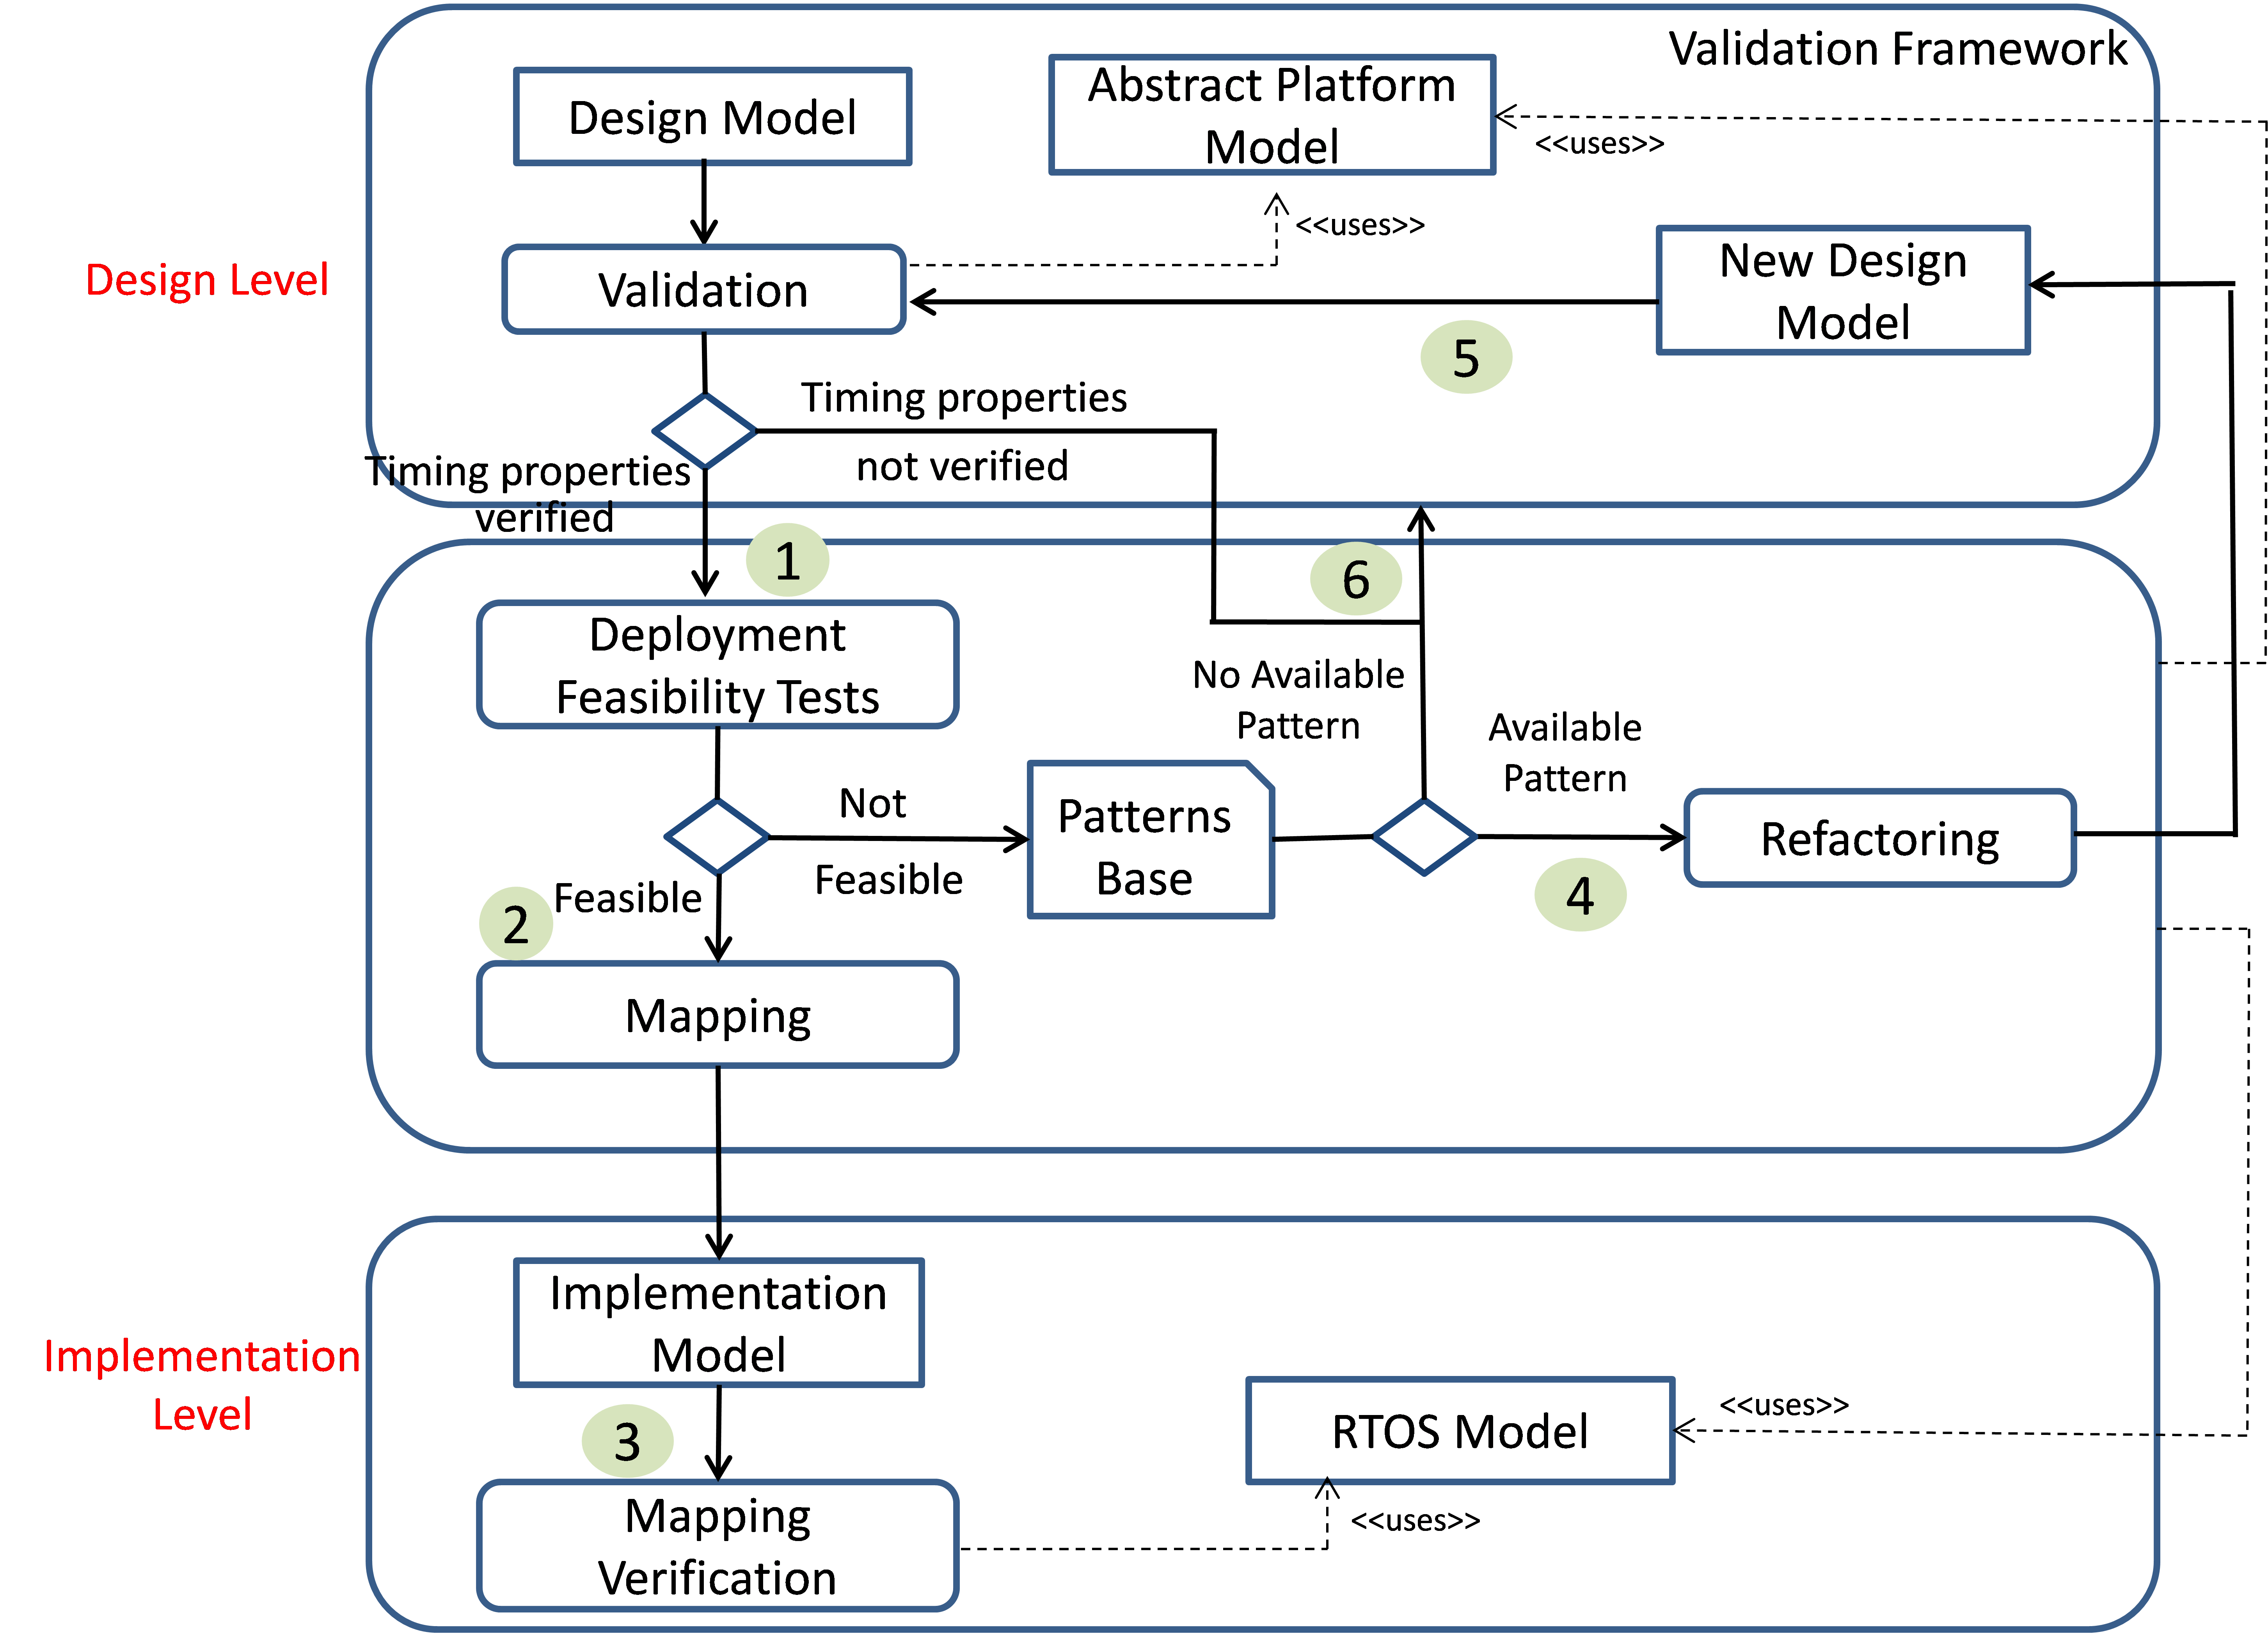
\includegraphics[width = 8cm,height=6cm]{Pic/process}
\caption{Design Refinement Method Overview}
\label{myprocess}
\end{figure}
\vspace{-0.5cm}
\\Our objective is to ensure a correct transition from a correct design model, to the implementation model while preserving its timing properties. Indeed, we are interested in the semantics of the software platform resources involved during the refinement. To this end, in previous work \cite {SEAA}, we have proposed to integrate two steps; deployment feasibility tests (1) step and mapping step (2). The first step defines a set of feasibility tests to verify whether the design choices are implementable on the target RTOS. When no feasibility concerns are raised, the mapping step generates the appropriate RTOS-specific model. These two steps are based on an explicit description of an abstract platform used for validation \cite{SEAA} and a concrete platform which corresponds to the RTOS. The mapping verification step (3) previously introduced in \cite{models}, defines the set of properties that must be verified to confirm the correctness of the refinement. 
\\In this paper, we are addressing the case where the design model is not implementable on the target RTOS. In that situation, the deployment feasibility tests step generates a warning to highlight that the input model is not implementable for a particular reason. One objective of our work is to guide the designer by proposing solutions whenever the refinement is not feasible. To this end, we create a \emph{pattern base} which collects a set of predefined patterns. Each pattern aims at solving a particular deployment problem in the case where some particular assumptions are fulfilled by the considered design model. 
Therefore, when a problem is detected, we verify if a pattern corresponding to this problem exists in the pattern base. If it is not the case, our framework generates an error to inform the designer that the design model is not implementable on the selected RTOS and that no solution is available to solve the problem. 
Otherwise, when a pattern is available (4), we perform the re-factoring of the design model by applying this pattern. This re-factoring must guarantee two points: (1) the portability and (2) the preservation of timing properties. Regarding the first point, even if the re-factoring of the design model is performed to handle the deployment problems related to the target RTOS, it must still independent from the latter: the resulting design model (denoted new design model in Fig.\ref{myprocess}) is also a PIM. In order to ensure the second point, the new design model must be revalidated (5). After performing the revalidation, if the timing properties are not verified, an error is generated to mention that the model is not implementable and no solution is available (6).  

\subsection {Design Model Formalization}
We assume that the considered real-time design model consists of \textit{m} \emph{periodic} tasks that we denote by $M = \{T_1,T_2,\ldots,T_m\}$ running in a single-processor system. Each task $T_i$ is defined by a set of parameters deducted from the high-level model (functional model) and the architectural choices enabling thus the timing validation. Indeed, a task $T_i$ is characterized by its priority $p_i$, its execution time $c_i$  which is considered as input in our case, its activation period $P_i$ supposed to be an integer in this paper and its deadline  $D_i$ that represents the time limit in which a task must complete its execution. We assume that 0 is the highest priority level and that tasks may share the same priority level. Let us denotes as \emph{n} the number of distinct priority levels used in the architectural model for validation $(n \leq m)$ and with  \emph{N}  the number of distinct priority levels allowed by the platform for the considered application. 



The architectural model consists also of a set of software resources $R =\{R_1,R_2,\ldots,R_\ell \}$ that can be shared between one or several tasks (e.g. a mutex to access a critical section). We denote $c_{R_i,T_j}$ the worst-case time for the task $T_j$ to acquire and release the lock of the resource $R_i$ in case of no contention. Let us remark that $c_{R_i,T_j}$ is considered as an input and that $c_{R_i,T_j} \leq c_j$. Due to the presence of shared resources, a task is also characterized by a blocking time $B_i$. The blocking time accounts for the time a higher-priority task has to wait, before acquiring the lock, since a lower-priority task owns this lock. The computation of this term depends on the synchronization protocol used to implement the access to the shared resource. In this paper, we suppose that Priority Ceiling protocol(PCP) \cite{PCP} is used as a synchronization protocol to avoid unbounded priority inversion and mutual deadlock due to wrong nesting of critical sections. In this protocol each resource $R_i$ is assigned a priority ceiling $\pi_i$, which is a priority equal to the highest priority of any task which may lock the resource. The expression used to compute the blocking time for the PCP protocol is given just below: 
\begin{equation}
\footnotesize{B_{i} = \max_{T_j \in HP ,R_k \in R}\{ c_{R_k,T_j} : p_{j} < p_{i} \ and \ \pi_{k} \geq p_{i}\}}
\label{eq:blockingTime}
\end{equation}


We perform Rate-Monotonic (RM) response time analysis \cite{RMA}. The analysis results correspond to the computation of the processor utilization U and the response time $Rep_i$ of the different tasks in the model. The model satisfies its timing constraints if and only if $U \leq 1$ and $\forall i \in \{1..m\}$ $Rep_i \leq D_i$. The expressions used to compute U and $Rep_i$ are given just below, where $HP_j$ represents the set of tasks with priority higher than $T_j$.
\begin{equation}
\footnotesize{U= \sum_{T_i \in M} \frac{c_i}{P_{i}}}
\label{eq:Utilization}
\end{equation}
\begin{equation}
\footnotesize{Rep_{i} = {c_i} + B_{i} + \sum_{T_j \in HP_j} \left\lceil \frac {Rep_{i}}{P_j} \right\rceil * {c_j} } 
\label{eq:responseTime}
\end{equation}
\begin{figure}[h]
\centering
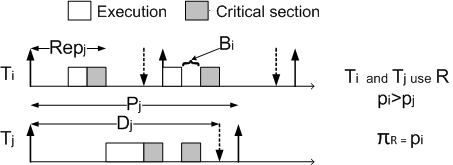
\includegraphics[height=2.5cm]{Pic/RT}
\caption{Real-Time Concepts}
\label{RT}
\end{figure}
\vspace{-0.2cm}
Fig.\ref{RT} shows an example of execution of two periodic tasks ($T_i$ and $T_j$) sharing the resource $R$. The priority ceiling of $R$ is equal to the priority of $T_i$ as it is the highest.Up-raising arrows represent the instants of tasks activation, for their part, down-raising arrows determine the deadline for each task activation. The response time to an activation is defined as the time between the activation and the completion instants. We also show the blocking time $B_i$ of the task $T_i$ resulting from the utilization of $R$ by $T_j$.
\\In addition, each task implements a set of functions that we denote by $ f \subset F/ card (f) \geq 1$ such as F is the set of functions defined by the application (from the functional model). 

\section{Problem Statement and Solution}
In this section, we identify the case where the Distinct Priority Merge Pattern (DPMP) must be applied. Then the proposed solution is detailed. 
\subsection{Problem Statement}
This pattern is automatically applied on the design model when the \emph{Deployment Feasibility Tests }step detects that the number of distinct priority levels used in the architectural model exceeds the number allowed by the RTOS for the considered application (i.e. $n > N$). The resulting design model after applying this pattern must still verifying the timing requirements as specified in section 2.2.  
\subsection{Solution Description}
In order to solve the problem (i.e. $n > N$), we propose to reduce \textit{n} to be equal to \textit{N} by merging tasks having distinct priority levels. This operation is repeated until the number of distinct priority levels becomes equal to \textit{N}. However, the proposed solution must preserve:
\begin{enumerate}
\item The high level specification i.e. the activation rate of the different functions defined in the specification must be preserved. 
\item The real-time constraints i.e. the response time of the all considered tasks is lower than their deadline. 
\end{enumerate} 
Let us consider an initial model $M =\{T_1,T_2,….,T_m\}$ defining \emph{m} tasks and \emph{n} distinct priority levels $(n \leq m)$. Let us consider also two tasks $T_i$ and $T_j \in M$, each task is defined by a set of parameters; $T_i=(p_i,C_i,P_i,D_i,B_i,f_i)$ and $T_j=(p_j,C_j,P_j,D_j,B_j,f_j)$ such as  $p_i \ne p_j$, $P_j \geq P_i$ and $f_i,f_j$ corresponds to the functions implemented respectively by $T_i$ and $T_j$. We denote by $T'_i$ the  task resulting from merging these two tasks such as $T'_i =(p'_i,C'_i,P'_i,D'_i,B'_i,f'_i)$. Consequently, the resulting model $M'$ consists of \emph{m-1} tasks and \emph{n-1 }distinct priority levels.The obtained task $ T'_i$ is described in Fig.\ref{fig:solutiondescriptionA}.


\begin{figure}[h]\label{fig:solutiondescription}
\centering
\mbox
{
\subfigure[Solution without considering harmonic tasks]
{
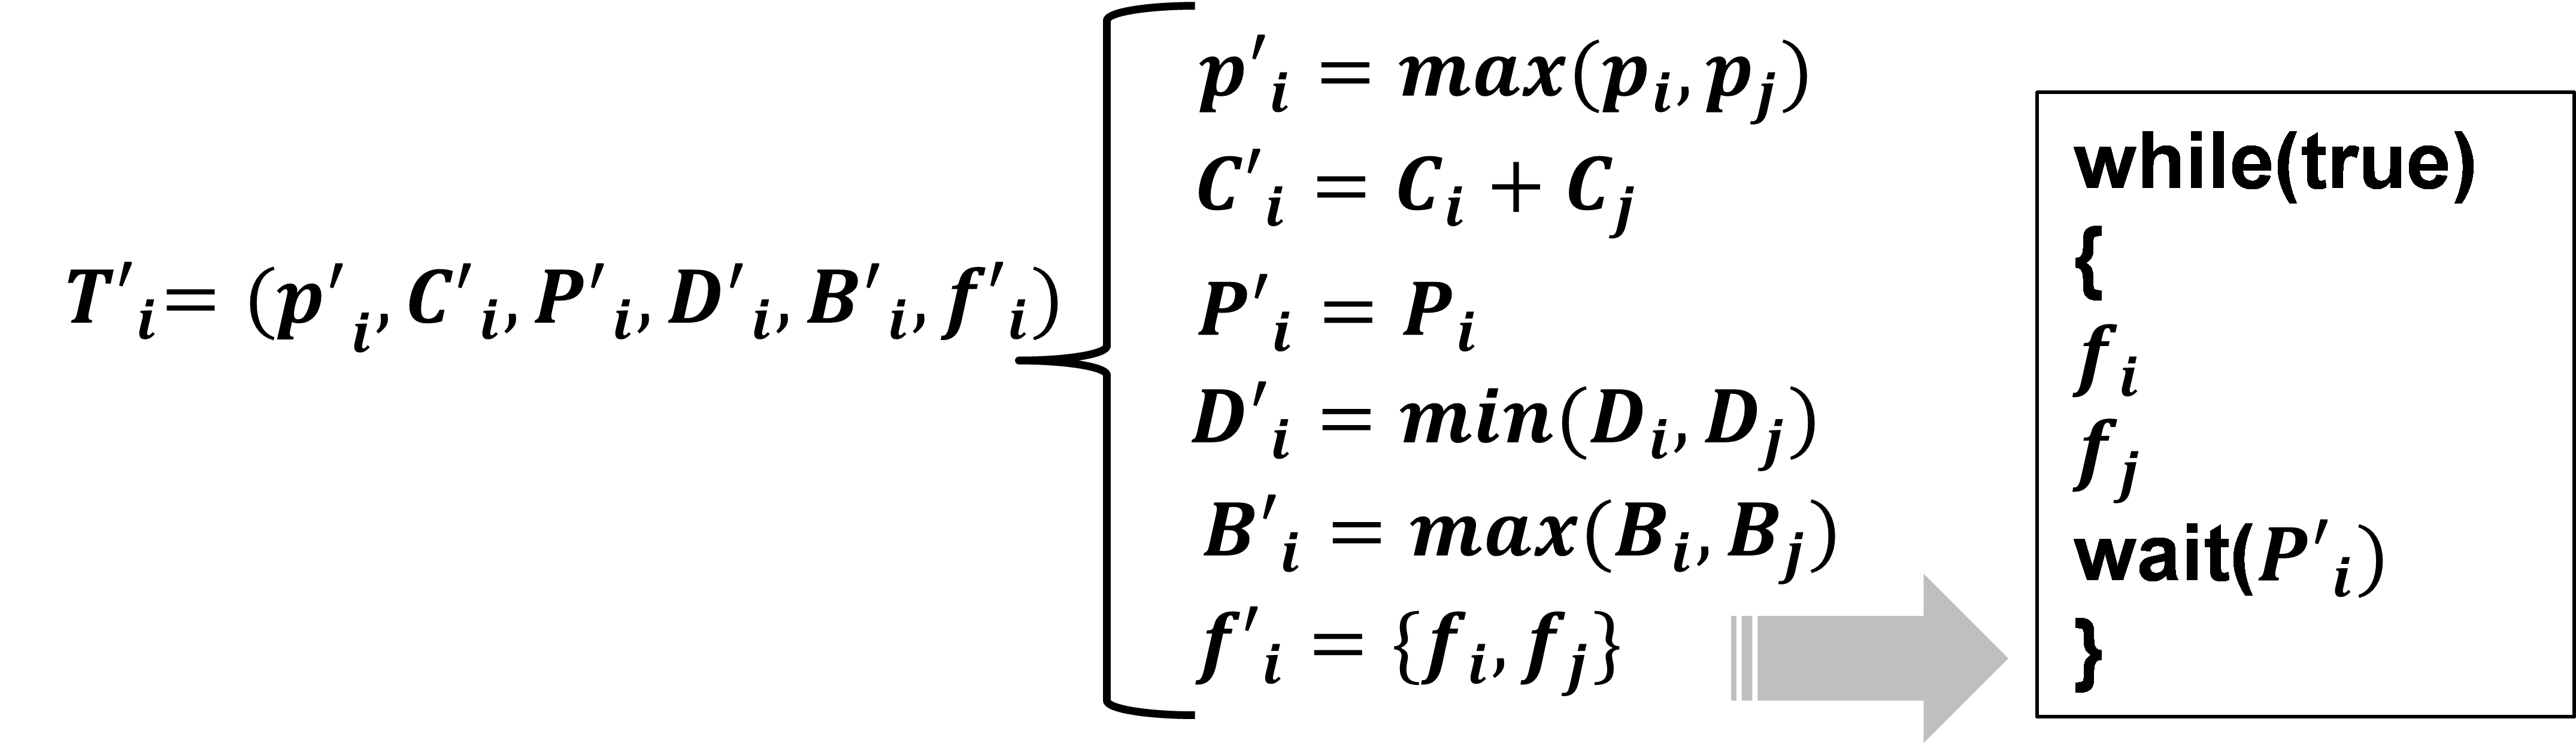
\includegraphics[width = 6cm]{Pic/MergeModel}
\label{fig:solutiondescriptionA}
}
\subfigure[Solution with harmonic tasks consideration]
{
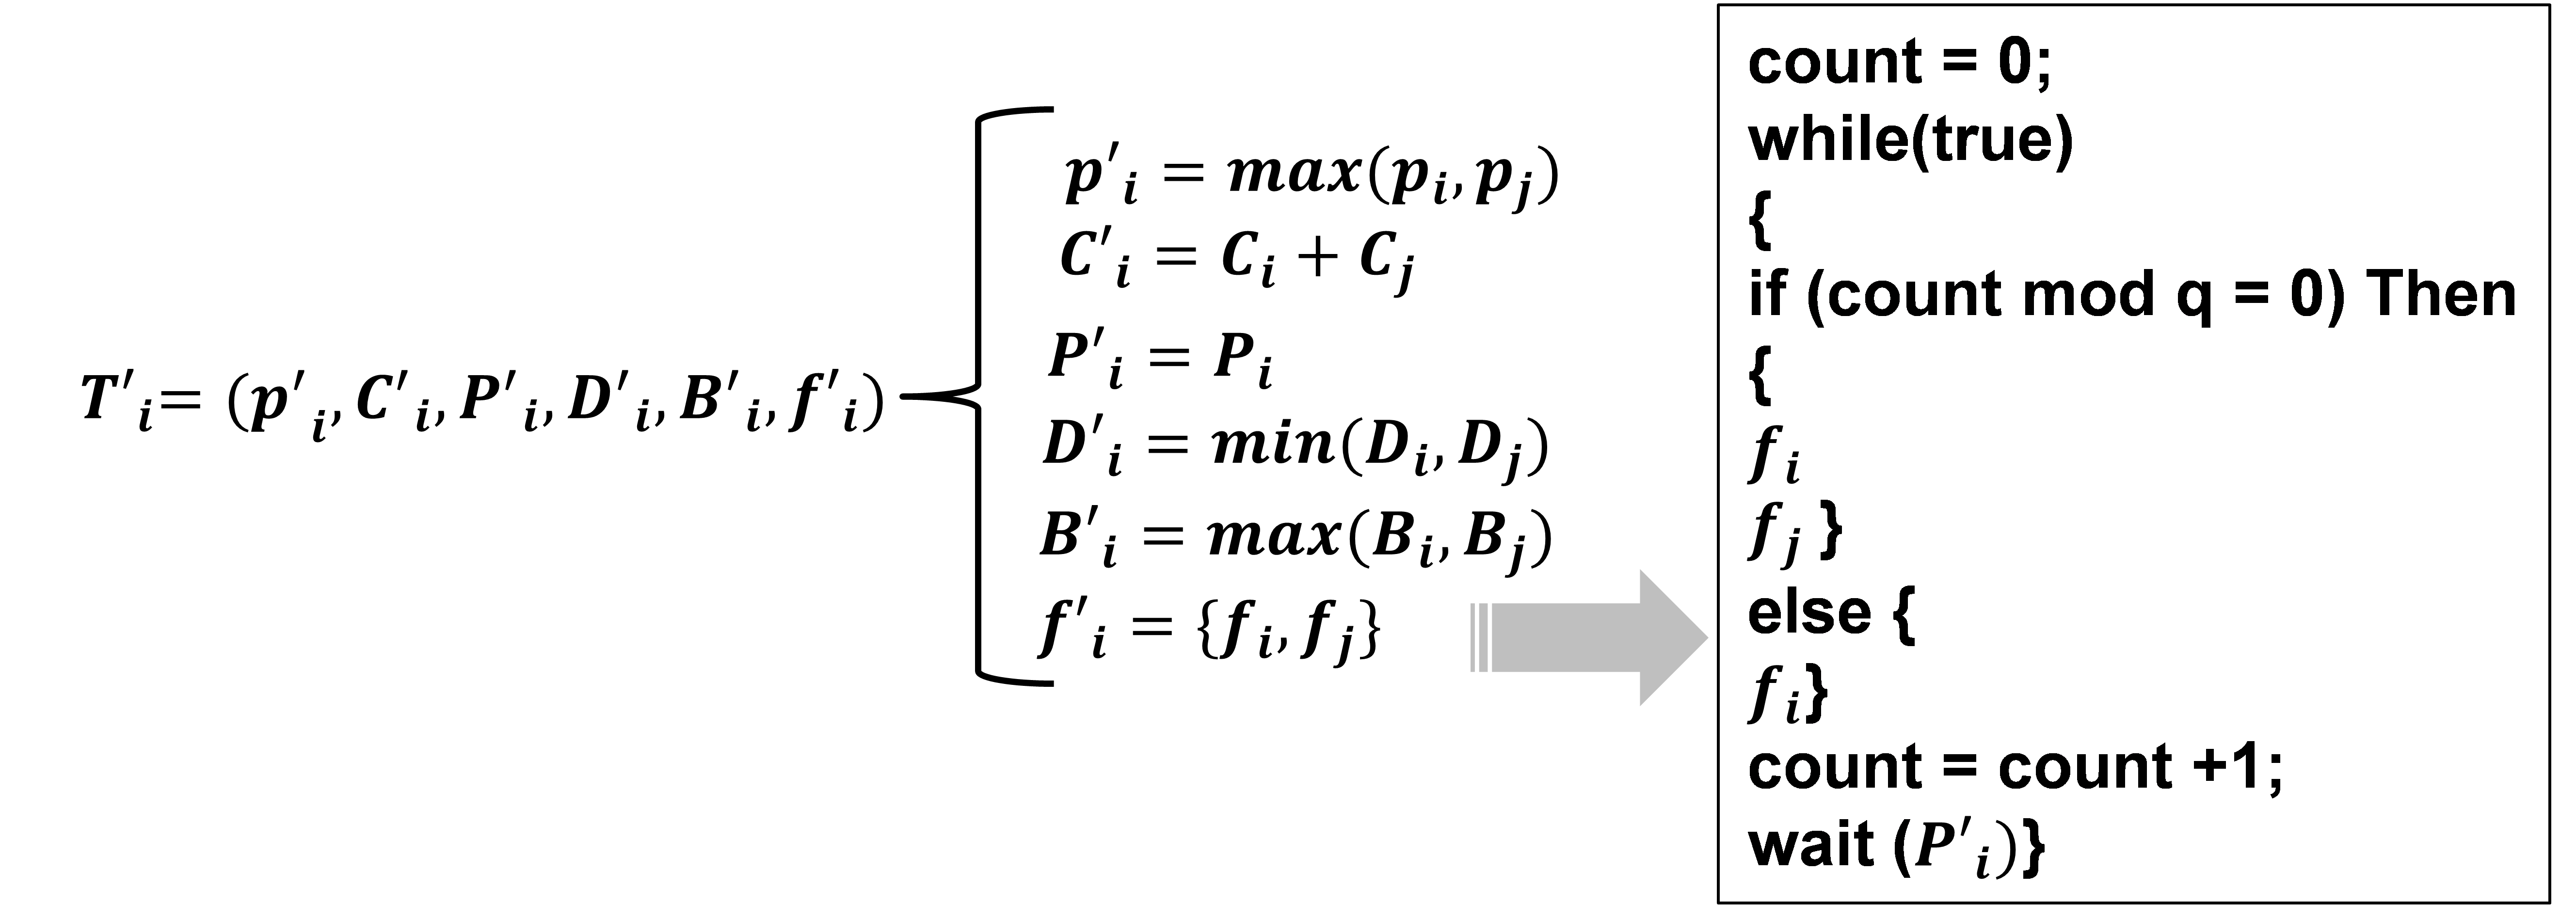
\includegraphics[width =6cm]{Pic/MergeModelbis}
\label{fig:solutiondescriptionB}
}
}
\caption{Solution Description}
\end{figure}
%\begin{figure}[h]
%\centering
%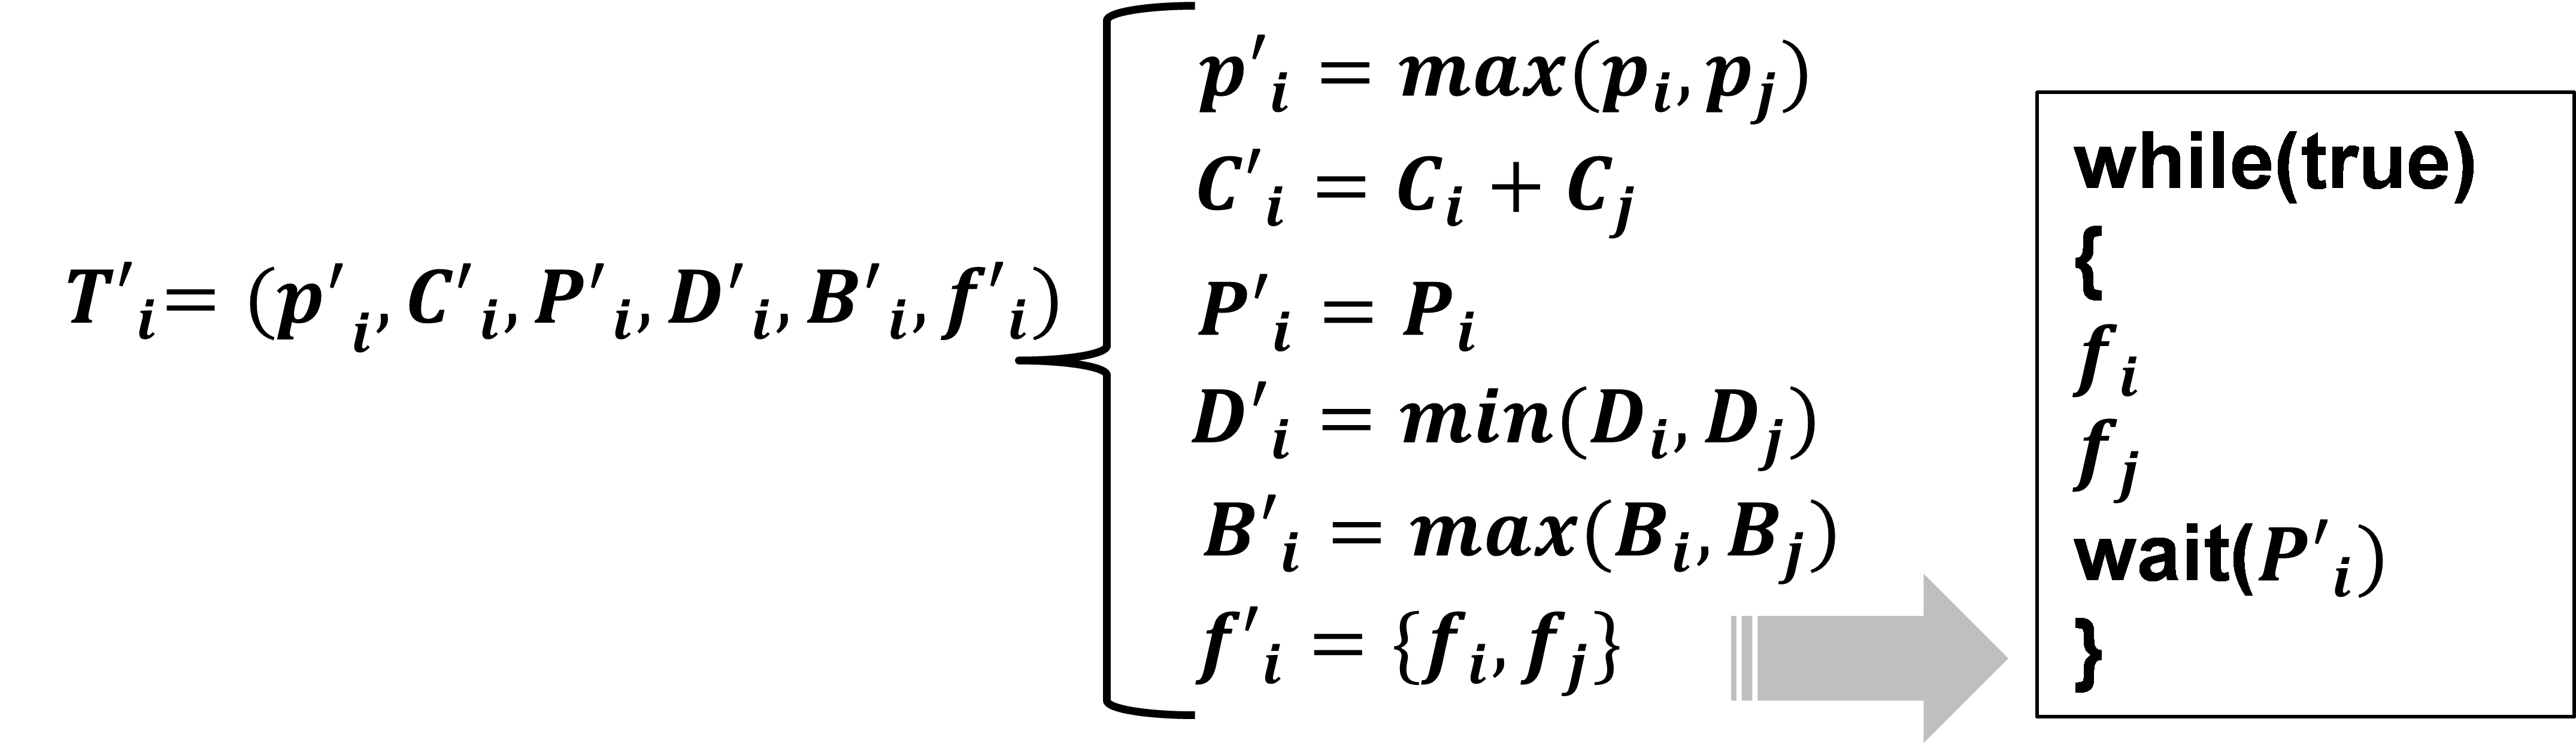
\includegraphics[height=3cm]{Pic/MergeModel}
%\caption{Model-Driven Approach}
%\label{process}
%\end{figure}


The problem with the resulting model described in Fig.\ref{fig:solutiondescriptionA} where one of the two merged tasks will be executed with a rate different from the one defined in the high level specification and thus the first constraint (1) previously defined will be violated. In order to avoid this problem, we consider also in the solution that only \emph{harmonic tasks} may be merged (i.e. two tasks $T_i$ and $T_j$ are harmonic if and only if ($P_j\quad mod \quad P_i = 0$). 
By considering this additional assumption ($\frac{P_j}{P_i} = q $ with q in an integer), the period of the resulting task which corresponds to minimum of the two periods will be equal to $P_i$ and the implementation of $f'_i$ will be modified in such a way that the execution rate of the two functions is preserved. The new solution is presented in Fig. \ref{fig:solutiondescriptionB}.
%\begin{figure}[h]
%\centering
%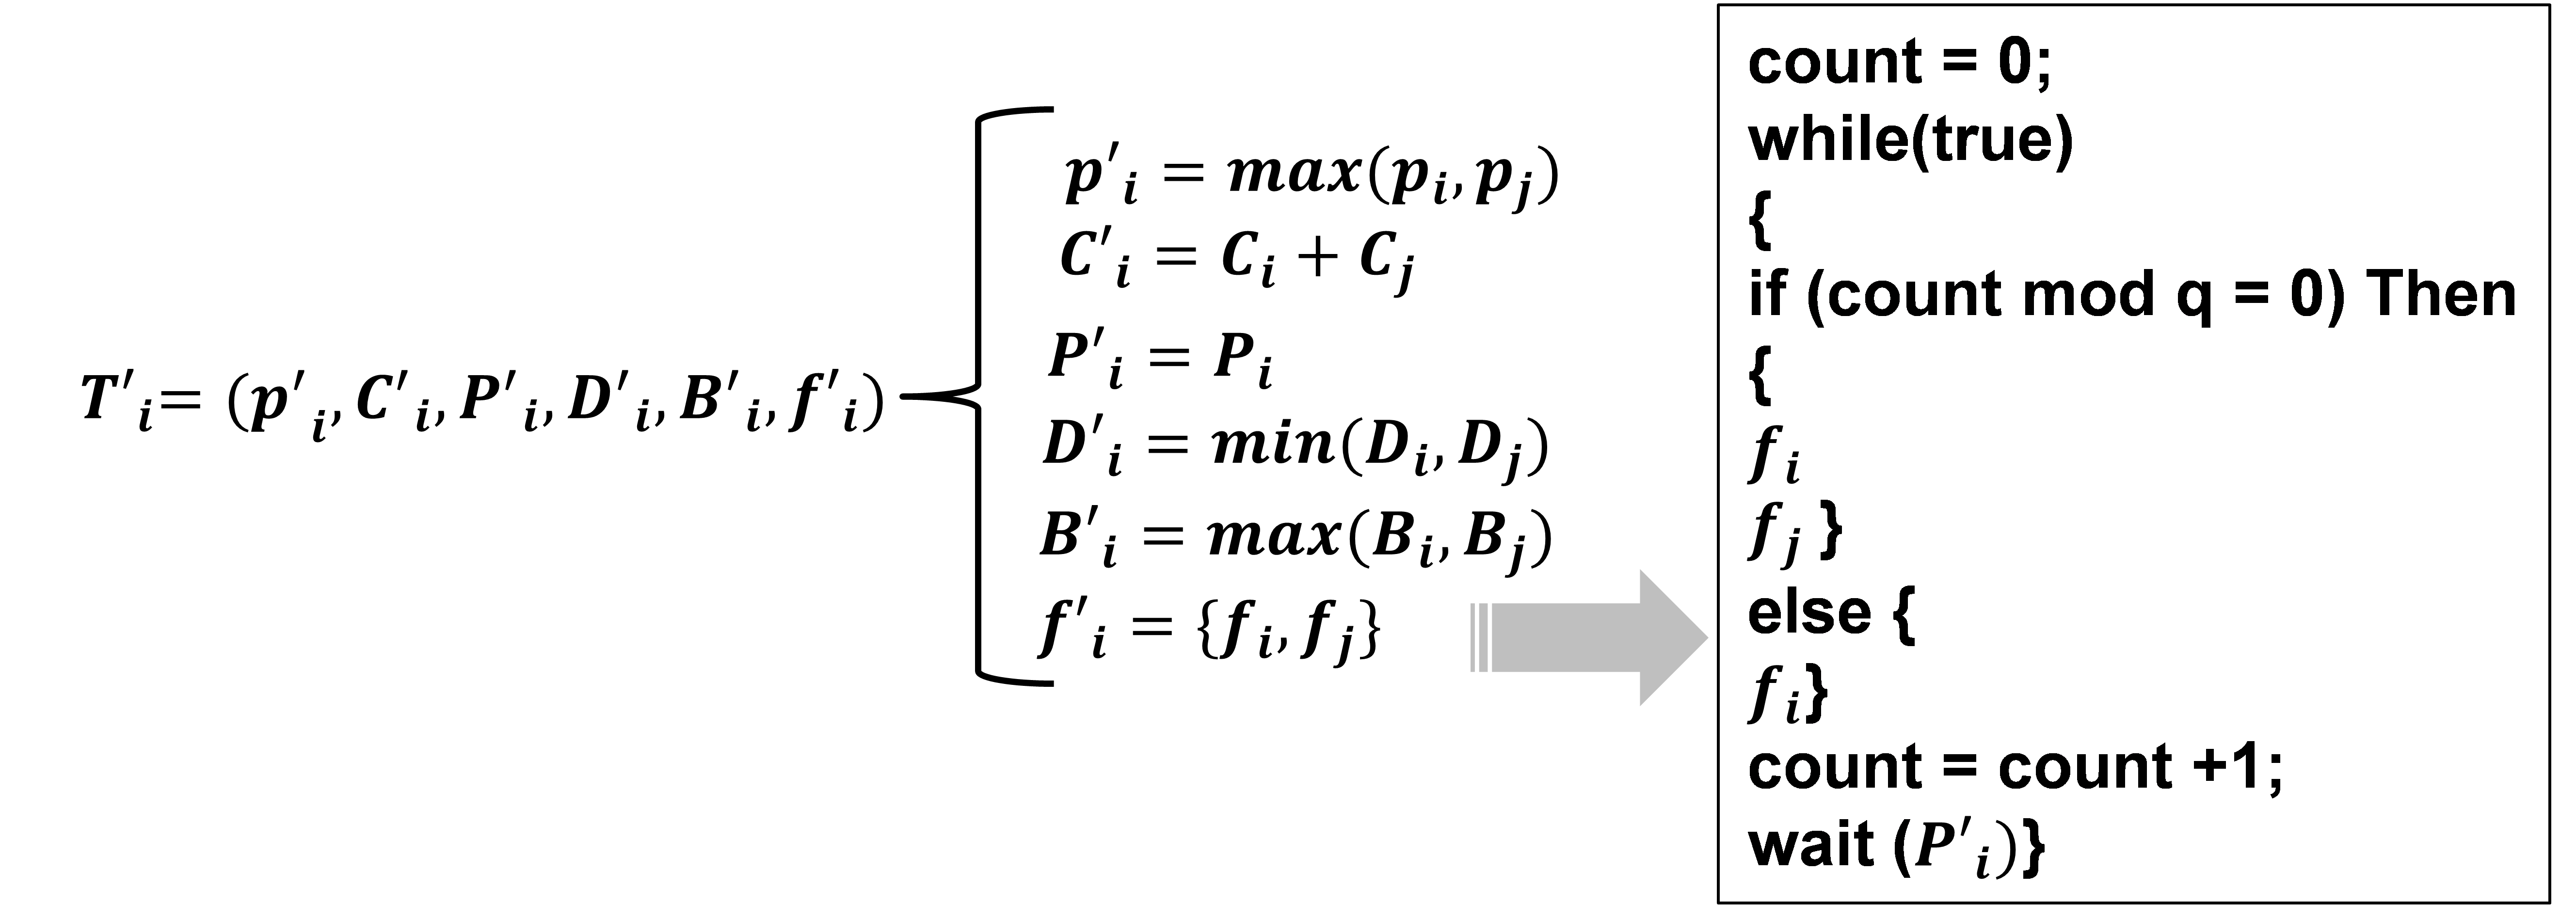
\includegraphics[height=3cm]{Pic/MergeModelbis}
%\caption{Model-Driven Approach}
%\label{process}
%\end{figure}
\\In order to guarantee the second constraint (2), we have to re-validate the model after merging the tasks in order to verify whether the new design model still satisfy the timing constraints.

\section{DPMP Formulation}
This section presents an algorithmic description of the previously proposed solution. Then, we show the limitations of this method and we propose a MILP formulation of the DPMP pattern.  
\subsection{Heuristic Method}
Algorithm 1 just below corresponds to an algorithmic description of the DPMP pattern.
\begin{algorithm}[h]
\DontPrintSemicolon
\begin {scriptsize}
\KwIn{ \\$M_a$: Design Model describing the application \\
$N$ : The number of distinct priority levels allowed by the RTOS for the considered application \\ 
Ref-Period : A reference period used to detect harmonic tasks}
\KwOut{ \\$M_{Res}$: New design model after reducing the number of priority levels\\}
\textbf{Notations:}\\
\textit {Ref-Task}: The reference task with the lowest value of period \\
\textit {H-Tasks}: The set of tasks which are harmonic with \textit{Ref-Task}\\
\textit {n}: The number of distinct priority levels used in the design model \\
\Begin{
  $M_{Res} \longleftarrow M_a$\\
  \textit {n $\longleftarrow$ \textit{getPriorityLevelsNumber($M_a$)}} \\
  \textit{Ref-Task} $\longleftarrow$ \textit{getMinPeriod($M_a$, Ref-Period)} \\
 
  \If {(\textit{Ref-Task} $\ne$ null)}
  {
    \For {($i_s \in M_a$ / $i_s$ is a periodic task)} 
    {
      \If {(IsInteger(period($i_s$), period(Ref-Task))} 
      {
         \If {(priority($i_s$)$\ne$ priority(Ref-Task))}
         {
           add($i_s$, H-Tasks)                                          
         }
      }
    }
    \If {(SizeOf(H-Tasks) $\leq$ 1)}
    {
      Ref-Period $\longleftarrow$ period(Ref-Task)
      DistinctPriorityMergePattern($M_a$,$N$,Ref-Period) 
    }
    \Else
    {
      \If {(n $\succ$ N)}
      {
       $M'_a$ $\longleftarrow$ Merge(H-Tasks[1],H-Tasks[2])\\
       OK $\longleftarrow$ Re-Validate ($M'_a$)\\
       \If {(Ok = true)}
       {
         $M_{Res}$ $\longleftarrow$ $M'_a$\\
         DistinctPriorityMergePattern($M_{Res}$,$N$,Ref-Period)
       }
      }
    }
  }
  return $M_{Res}$
  }
\caption{DistinctPriorityMergePattern\label{pattern}}
\end{scriptsize}
\end{algorithm}
This algorithm merges recursively tasks in pairs. After each merge, this algorithm performs a re-validation to verify the timing properties. 
The algorithm ends, when the number of distinct priority levels used in the resulting model is equal to the number authorized by the target RTOS or when there is no harmonic tasks in the model. The complexity of this algorithm is linear and it depends on the number of tasks in the initial model. 
\subsubsection{Heuristic Method Limitations}
The problem of merging tasks with the objective to reduce the number of distinct applicative priority levels is \emph{a combinatorial problem}. In fact, the solution depends on the application (i.e. \emph{n} and the period of the different tasks) and the target RTOS. Consequently, the heuristic method presented in previous section is not always able to find the solution. 
\\Let's consider an initial model $M =\{T_1,T_2,T_3,T_4\}$. Each task is characterized by a set of parameters such as $T_1=(1,4,10,10,0,f_1)$, $T_2=(2,5,20,20,0,f_2)$, $T_3=(3,2,30,30,0,f_3)$ and $T_4=(4,1,60,60,0,f_4)$.The initial processor utilization is evaluated to 73,33 \%.
All the tasks in this model are independent and have distinct priority levels (n=4). We can notice that task $T_1$ is harmonic with all the other tasks and also $T_2$, $T_3$ are harmonic with $T_4$. In addition, we suppose that the target RTOS authorizes only \emph{two} priority levels for this application (N=2). 
\begin{table}[!h]
\caption{Example: Possible Solutions and Utilization Estimation}
\label{table1}
\centering
   \begin{tabular}{ | l || c |}
     \hline
     Possible Solutions & Utilization \\
     \hline
     $M_1 =(\{T_1,T_2\},\{T_3,T_4\}$) &  100\% \\
     \hline
     $M_2 =(\{T_1,T_3\},\{T_2,T_4\}$)& 90\% \\
     \hline
     $M_3 = (\{T_1,T_2,T_3\},T_4$) & 111,67\%\\
     \hline
     $M_4=(T_2,\{T_1,T_3,T_4\})$ & 95\% \\
     \hline
     $M_5= (T_3,\{T_1,T_2,T_4\})$ & 106,66\% \\
     \hline
   \end{tabular}
\end{table}


As a result, for this particular example, 5 solutions are possible. These solutions are presented in Table 1. 
For the first solution for example, we choose to merge $T_1$  and $T_2$  from one side and $T_3$  and $T_4$  from the other side in order to obtain the model $M_1$ consisting of just two tasks and thus two distinct priority levels. For this particular example, the heuristic method didn't find a feasible solution as it found  $M_3$ which is not feasible due to analysis issues (utilization 111,67\%$\succ$ 100\%). Therefore, this method is not always effective. From these considerations, an appropriate method must be considered to solve this problem. This method must be able to confirm whether a solution for each particular problem (application and RTOS) exists. In addition, when many solutions are available, this method should find one which costs less performance degradation. In next section, we propose a MILP formulation of this problem.

\subsection{MILP Formulation}
In order to ensure a reliable implementation of the problem taking into consideration the different constraints already mentioned (timing requirements, application…), we propose in this section a MILP formulation of our problem. MILP techniques define an objective function which corresponds to a formulation of the considered problem. This formulation is interpretable by a solver that seeks to find a solution for this problem under a set of defined constraints. 

\subsubsection{Objective Function}
Expression (\ref{eq:1}) defines the objective function for our problem. We denote by $m$ the number of tasks in the initial model. $Merge$ is a boolean variable used to mention whether two tasks are merged. More in detail, if $Merge_{i,j}$ is equal to 1, the merge corresponds to the situtation in which $T_i$ absorbs $T_j$, then $T_i$ augments its worst-case execution time by adding the worst-case execution time of $T_j$, while $T_j$ is deleted from the model. Let us note that more than one task can be absorbed by another task. 
The objective function aims at maximizing the number of merge while minimizing the processor utilization. 
\begin{equation}
\footnotesize{ \mathrm{maximize : \sum_{i,j \in \{1..m \}}{Merge_{i,j}} - Utilization }}
\label{eq:1}
\end{equation}
\subsubsection{Merging Situations Constraints}
The objective function aims at maximizing the number of merge, however this function should be aware of some constraints that limit the exploration space and eliminate non meaningful merging situations. These constraints are presented just below: 
\begin{equation}
\footnotesize{\mathrm{n - \sum_{i,j \in \{1..m \}}{Merge_{i,j}} = N}}
\label{eq:2}
\end{equation}
\begin{equation}
\footnotesize{\mathrm{\forall{i,j \in \{1..m\}}, Merge_{i,j} =0 \quad if \quad (isHarmonic_{i,j}=0) \quad or \quad (p_{i} =p_{j})} }
\label{eq:3}
\end{equation}
%\begin{equation}
%\mathrm{\forall{i,j \in \{1..m\}}, Merge_{i,j} =0 \quad if \quad  (p_{i} =p_{j}) \quad and \quad (i \ne j)}
%\end{equation}
%\begin{equation}
%\mathrm{\forall{i,j \in \{1..m\}}, Merge_{i,j} =0  \quad if \quad   (i = j)} 
%\end{equation}
\begin{equation}
\footnotesize{\mathrm{\forall{j \in \{1..m\}}, \sum_{i\in \{1..m\} \wedge  i  \neq j } Merge_{i,j} \leq 1}} \ ; \ \footnotesize{\mathrm{\forall{i,j,k \in \{1..m\} \wedge j,k  \neq i }, Merge_{i,j} +  Merge_{k,i} \leq 1} } 
\label{eq:4}
\end{equation}
%\begin{equation}
%\footnotesize{\mathrm{\forall{i,j,k \in \{1..m\}}, Merge_{i,j} +  Merge_{j,k} \leq 1} } 
%\end{equation}
In constraint (\ref{eq:2}), n and N represent two input parameters defined previously in section 2.2. This constraint means that we have to maximize the number of merged tasks and thus minimize the number of distinct priority levels used in the design model until the number authorized by the RTOS. Indeed, this Equation serves as a bound for the objective function (i.e. the number of merge). Constraint (\ref{eq:3}) defines a new input parameter which is \emph{isHarmonic}, this parameter is used to mention if two tasks are harmonic. Thus if the value of $isHarmonic_{i,j}$  is equal to 1, then the corresponding tasks $T_i$ and $T_j$ have harmonic rates. Consequently, this constraint avoids the merge of non-harmonic tasks and avoids also the merge of tasks having equal priority levels($p_i=p_j$). Finally, the constraints in (\ref{eq:4}) are used to avoid a non-meaningful situations which corresponds to the merge of a task already merged. In particular, the first contraint assures that a task $T_j$ can be absorbed by at most one other task, and the second constraint states that either  a task absorbs another task or it is absorded by another task. 
\\We define also a new boolean variable that we denote by TASKS and which refers to the resulting task model after merging the different tasks. Therefore, constraint (\ref{eq:5}) is defined to create the new obtained model. In fact, when $Merge_{i,j}$ is equal to 1, $TASKS_{j}$ will be equal to 0 and $TASKS_{i}$ will be equal to 1 (thanks to constraints \ref{eq:4}). This constraint is defined as follows:   
\begin{equation}
\footnotesize{\mathrm{\forall{j \in \{1..m\}}, TASKS_{j} = 1 - \sum_{i \in \{1..m\}}Merge_{i,j} }}
\label{eq:5}
\end{equation}
\subsubsection{Real-Time Constraints}
The constraints defined in this section are related to real-time requirements. Indeed, the model obtained after applying the merge pattern should satisfy the timing constraints which are expressed in constraints (\ref{eq:6}) and (\ref{eq:7}). 
\begin{equation}
\footnotesize{\mathrm{\forall{i \in \{1..m\}}, Rep_{i} \leq D_{i} } }
\label{eq:6}
\end{equation}
\begin{equation}
\footnotesize{\mathrm{utilization \leq Max\_Utilization}  }
\label{eq:7}
\end{equation}
Constraint (\ref{eq:6}) ensures that the response times $Rep_i$ of the different tasks in the resulting model are lower or equal than their deadlines. Constraint (\ref{eq:7}) verifies whether the processor utilization is lower or equal than the maximum authorized utilization. %Now, we will define the different constraints used to compute the response time and the utilization. 
Constraint (\ref{eq:8}) gives the computation formula of $T_i$ response time while taking into consideration the different decisions of merge. 
\begin{equation}
\footnotesize{\mathrm{\forall{i \in \{1..m\}}, Rep_{i} = \delta_i + \theta_i + \beta_i }}
\label{eq:8}
\end{equation}
The first term of the expression (\ref{eq:8}) is $\delta_i$ which corresponds to the worst case execution time of the task $T_i$. This term is computed as follows: 
\begin{equation}
\footnotesize{\forall{i \in \{1..m\}}, \delta_i = TASKS_i *C_i + \sum_{j \in \{1..m\}} Merge_{i,j}*C_j }
\label{eq:9}
\end{equation}
The execution time of a deleted task will be equal to 0 since the term $TASKS_i$ is equal to 0 and  $\forall j \in \{1..m\}, Merge_{i,j}=0$. However, the execution time of a task resulting from the merge of different tasks will be equal to the sum of the execution times of these tasks. 
\\The second term in the expression is $\theta_i$ representing the overhead induced by the interferences of the task $T_i$ with the different tasks in the model having higher priorities. This variable is defined $\forall{i \in \{1..m\}}$ as the sum of two terms $\zeta_i$, $\gamma_i$ and it is defined just below:  
\begin{equation}
\footnotesize{\mathrm{\theta_i = \zeta_i + \gamma_i }}
\label{eq:10}
\end{equation}
\begin{equation}
\footnotesize{\mathrm{\zeta_i= TASKS_i * \sum_{\underset{j \in \{1..m\}}{ j \in{HP_i}}} TASKS_j *(\lceil \frac{Rep_i}{P_j}\rceil*C_j)}}
\label{eq:11}
\end{equation}
\begin{equation}
\footnotesize{\mathrm{\gamma_i= TASKS_i * [\sum_{\underset{j \in \{1..m\}}{ j \in {HP_i}}} TASKS_j *(\sum_{k \in \{1..m\}} Merge_{j,k} *\lceil \frac{Rep_i}{P_j}\rceil*C_k)]}}
\label{eq:12}
\end{equation}
The interference term is equal to 0 if the corresponding task is a deleted one ($TASKS_i$). Otherwise, this term computes the overhead resulting from the interferences of tasks $T_j / j \in HP_i$. This expression takes into consideration the different situations when higher priority tasks correspond to deleted ones ($TASKS_j$ in the expression) or tasks resulting from merging decision ($Merge_{j,k}$ in the expression). 
We notice that the expressions (\ref{eq:11}) and (\ref{eq:12}) are not linear and thus in order to be interpretable by the solver these expression must be linearized. For instance, the linearization of the expression (\ref{eq:11}) is given by the following constraints: 
\begin{equation}
\footnotesize{\mathrm{\forall{i,j \in \{1..m\}}, 0 \leq X_{i,j}- (\frac{Rep_i}{P_j})}< 1}
\label{eq:13}
\end{equation}
\begin{equation}
\footnotesize{\mathrm{\forall{i,j \in \{1..m\}}, Y_{i,j} \leq X_{i,j}}} \ ; \
\footnotesize{\mathrm{ Y_{i,j} \leq M*TASKS_j}} \ ; \
\footnotesize{\mathrm{ X_{i,j} - M*(1-TASKS_j) \leq Y_{i,j}}}
\label{eq:14}
\end{equation}
%\begin{equation}
%\footnotesize{\mathrm{\forall{i,j \in \{1..m\}}, Y_{i,j} \leq M*TASKS_j}}
%\end{equation}
%\begin{equation}
%\footnotesize{\mathrm{\forall{i,j \in \{1..m\}}, X_{i,j} - M*(1-TASKS_j) \leq Y_{i,j}}}
%\end{equation}
In order to linearize the expression (\ref{eq:11}), we define new constraints (\ref{eq:13})  (\ref{eq:14}) and 2 additional variables $X$ and $Y$. The constraint (\ref{eq:13}) permits to compute the term $\lceil \frac{Rep_i}{P_j}\rceil$, however the constraints in (\ref{eq:14}) are defined to determine the value of  $(TASKS_j)*\lceil \frac{Rep_i}{P_j}\rceil$. Eventually, the constraints in (\ref{eq:15}) and (\ref{eq:16}) are used to compute the final value of $\zeta_i$, $\forall i \in \{1..m\}$.  
\begin{equation}
\footnotesize{\mathrm{\forall{i \in \{1..m\}},  \zeta_i \leq \sum_{\underset{j \in \{1..m\}}{ j \in {HP_i}}} Y_ {i,j} *C_j }} \ ; \ \footnotesize{\mathrm{  \zeta_i \leq M*TASKS_i }}
\label{eq:15}
\end{equation}
%\begin{equation}
%\footnotesize{\mathrm{\forall{i \in \{1..m\}},  \zeta_i \leq M*TASKS_i }}
%\end{equation}
\begin{equation}
\footnotesize{\mathrm{\forall{i \in \{1..m\}},[ \sum_{\underset{j \in \{1..m\}}{ j \in {HP_i}}} Y_ {i,j} *C_j] - M*(1-TASKS_i) \leq \zeta_i }}
\label{eq:16}
\end{equation}
\\Finally the third term in the expression of the response time $\beta_i$ represents the blocking time. This variable is computed as follows: 
\begin{equation}
\footnotesize{\mathrm{\forall{i \in \{1..m\}},  \beta_i = TASKS_i *BT_i }}
\label{eq:17}
\end{equation}
This term is equal to 0 if the task corresponds to a deleted task. Otherwise, the blocking time of the considered task is equal to $BT$ which is defined as follows: 
\begin{equation}
\footnotesize{\mathrm{\forall{i \in \{1..m\}}, \quad BT_i =}}
\left\lbrace
\begin{array}{ccc}
\footnotesize{\mathrm{B_i \quad if  \quad \sum_{i,j \in \{1..m\}} Merge_{i,j} =0}}\\
\footnotesize{\mathrm{\max_{j \in \{1..m\}} Merge_{i,j} * B_i   \quad Otherwise}}
\end{array}\right.
\label{eq:18}
\end{equation}
The term $B_i$ in expression (\ref{eq:18}) is an input parameter representing the blocking time of the task $T_i$. Consequently, if the considered task is not merged with other tasks in model ($\sum_{j \in \{1..m\}} Merge_{i,j} = 0$), the blocking time is kept the same. Otherwise, the blocking term corresponds to the maximum of the merged task blocking times. 
The processor utilization represents an important term in scheduling analysis. In fact, in order to confirm that the design model meets the timing constraints the following constraint must be verified: 
\begin{equation}
\footnotesize{\mathrm{Utilization \leq 1}}
\end{equation}
We define the Utilization term by the constraints just below:
\begin{equation}
\footnotesize{\mathrm{Utilization = \mu_1 + \mu_2}}
\end{equation}
\begin{equation}
\footnotesize{\mathrm{\mu_1 = \sum_{i \in \{1..m\}} TASKS_i * (\frac{C_i}{P_i})}} \ ; \ \footnotesize{\mathrm{\mu_2 = \sum_{i \in \{1..m\}} TASKS_i * \sum_{j \in \{1..m\}} Merge_{i,j}*(\frac{C_j}{P_i})}}
\end{equation}
%\begin{equation}
%\footnotesize{\mathrm{\mu_2 = \sum_{i \in \{1..m\}} TASKS_i * \sum_{j \in \{1..m\}} Merge_{i,j}*(\frac{C_j}{P_i})}}
%\end{equation}
Under these constraints, the objective function will seek for the best way to merge tasks (i.e. the optimized solution in terms of utilization) in order to reduce the number of used priority levels while ensuring the respect of timing properties. \\
Let's consider the same example previously introduced in section 4.1. Considering this problem, our linear program confirms that a solution exists and generates the following $Merge$ matrix: \\
%The considered design model $M =\{T_1,T_2,T_3,T_4\}$ consists of four independent tasks. Each task is characterized by a set of parameters such as $T_1=(1,4,10,10,0,f_1)$, $T_2=(2,5,20,20,0,f_2)$, $T_3=(3,2,30,30,0,f_3)$ and $T_4=(4,1,60,60,0,f_4)$.The initial processor utilization for this model is 73,33 \%. In the same way, we consider that the target RTOS supports just two distinct priority levels. Consequently, 
\begin{center}
$Merge$ = $ \begin{pmatrix}
0&0&1&0\\
0&0&0&1 \\
0&0&0&0\\
0&0&0&0\\
\end{pmatrix}$
\end{center}
This matrix shows that the solution considered by the solver is the merge of $T_1$ and $T_3$ and the merge of $T_2$ and $T_4$. The processor utilization of the resulting model is 90\%. Now if we compare this solution with the different possible solutions given in Table 1, we can conclude that the latter corresponds to $M_2$ which is the best one in terms of processor utilization.\\     
The solution generated by the linear program will be interpreted by our framework in order to provide the information to the designer on how the design model must be re-factored.
%This re-factoring permits to solve the problem of insufficient priority levels for the considered application while ensuring the respect of timing properties. 
\section{Experimental Results}

In this section, we present a set of experiments to test the effectiveness of the proposed pattern in terms of applicability and scalability. The experiments are carried-out on Intel Core i5-3360M processor running at 2.8 GHz with 4GB of cache memory. CPLEX is used as a MILP solver for the whole set of experiments. 
\\We define also a new parameter that we denote \emph{Cost}. This parameter references the \emph{performance loss} and is defined as the difference between the utilization evaluated on the initial model and the utilization evaluated on the model resulting from the application of the merge pattern in order to avoid non-implementable design models. Expression \ref{eq:cost} given just below defines this parameter:  
\begin{equation} \label{eq:cost}
\mathrm{Cost = Current_{utilization} - Initial_{utilization}}
\end{equation}
\subsection*{Extensibility at the Implementation Level}
We define the \emph{extensibility} as the capacity to integrate additional applications (or functions) on the same platform. In this section, we suppose that the first focus of the designer is to maximize extensibility at the implementation level even at the expense of some performance loss. For that achievement, the designer should determine the processor utilization authorised for his application that we denote by \emph{Max-Utilization }and the number of distinct priority levels denoted by N. This task is not trivial because it strongly depends on the application. The  previously described linear program provides a sort of guidance for the designer to help him determining one of these parameters by fixing the second. Therefore, two scenarios are considered: (1) the designer defines the maximum number of priority levels (N) that he wants to reserve for his application and asks the linear program to determine the minimum processor utilization necessary for this achievement.(2) the designer defines the maximum processor utilization (Max-Utilization) authorized for his application and asks the linear program to determine the minimum number of priority levels that are necessary to achieve such utilization.    
%\begin{itemize}
%\item the designer defines the maximum number of priority levels (N) that he wants to reserve for his application and asks the linear program to determine the minimum processor utilization necessary for this achievement. 
%\item the designer defines the maximum processor utilization (Max-Utilization) authorized for his application and asks the linear program to determine the minimum number of priority levels that are necessary to achieve such utilization. 
%\end{itemize} 
For scheduling issues, we suppose that the considered application is the first to be implemented on the platform and that the reserved priority levels are the higher ones.
\\In order to illustrate this idea, we consider an example of an architectural model describing an application; this model is given in table \ref{table3}. The design model consists of 6 tasks; each task is characterized by a set of parameters. Besides, the model defines also two shared resources $R_1$ and $R_2$; the resource $R_1$ is shared between the two tasks $T_1$ and $T_3$, however $R_2$ is shared between $T_2$ and $T_5$. After, the different design choices, the designer performs validation to verify the timing constraints. Validation results are also presented in table \ref{table3}; all the tasks meet their deadlines since their response times are  lower than their deadlines. The processor utilization for this model is evaluated to 39, 69\%. 
%\vspace{-0.2cm}
\begin{table}[h]
\caption{Example of an Architectural Model}
\label{table3}
\centering
   \begin{tabular}{ | c || c || c || c || c || c || c |}
     \hline
     Task  & Period  & Deadline  &	Wcet &	Priority  &	Blocking Time  &	Response Time  \\
     \hline
     $T_1$ & 10 &	10&	2&	0&	2&	4 \\
     \hline
     $T_2$	&20&	20&	2&	1&	2&	6 \\
     \hline
     $T_3$	&40&	40&	2&	2&	1&	7\\
     \hline
     $T_4$	&80	&80	&3	&3	&1	&10 \\
     \hline
     $T_5$	&160	&160	&1	&4	&0	&10 \\
      \hline
     $T_6$	&320&	320&	1&	5&	0&	13 \\
     \hline
   \end{tabular}
\end{table}  
\\Now let's consider the first scenario. For extensibility issues the designer wants to reserve just 3 priority levels for this application at the implementation level. To this end, he fixes the number N to 3 and asks the pattern to determine minimum processor utilization that should be reserved in that case. Then, the pattern generates the corresponding value which is equal to 46, 25\%.  For the second scenario, if the designer fixes the Max-Utilization to 45\%, the pattern determines that the minimum number of priority levels that should be reserved for such utilization is 4 (N=4).  
Fig.\ref{extensibility} illustrates the variation of the \emph{Cost} with regard to the \emph{extensibility }for the considered application.  
\begin{figure}
\centering
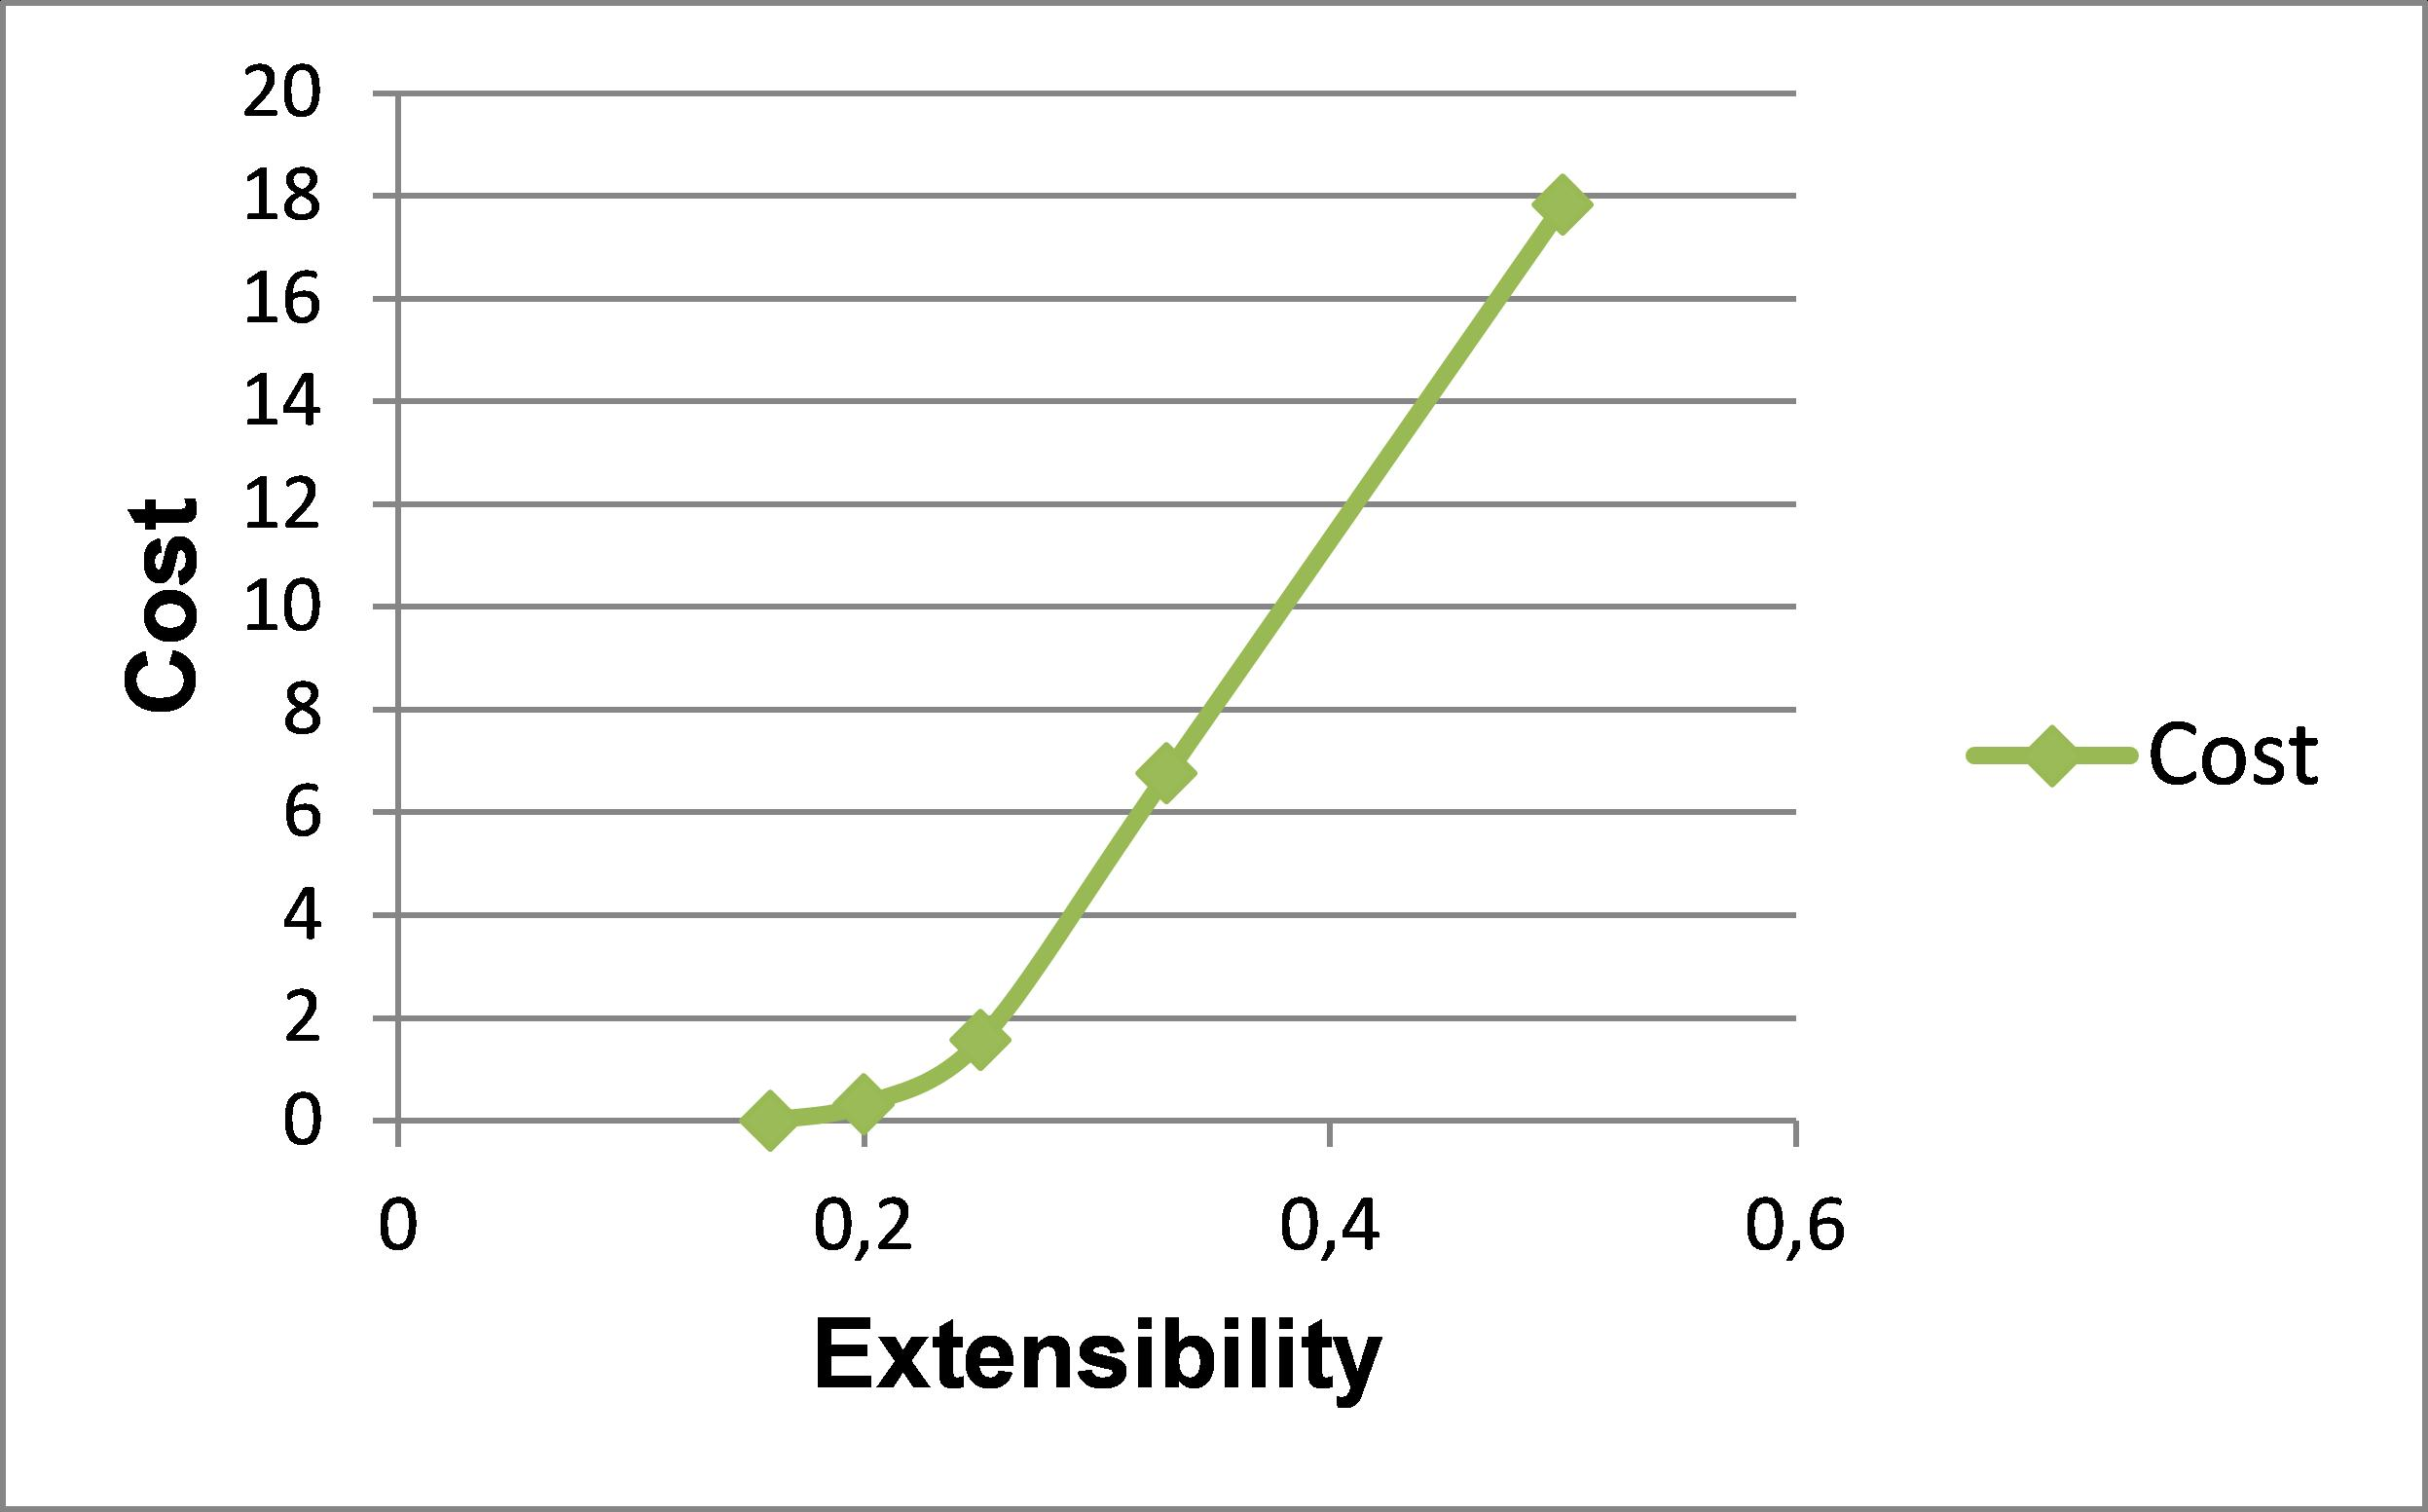
\includegraphics[height=3.5cm]{Pic/extensibility}
\caption{Cost Variation Versus Extensibility}
\label{extensibility}
\end{figure}
\\We have already mentioned that the extensibility is inversely proportional to the number of priority levels reserved at the implementation level. Hence, in the graph we evaluate the extensibility to be equal to $\frac{1}{N}$. We can conclude that the performance loss increases when the extensibility increases. 
\subsection*{Insufficient Priority Levels for Large Scale Applications} 
In this section, we are interested on the evaluation of the merge pattern on large scale systems. In that case, during the deployment phase, the problem of insufficient number of priority levels authorized by the target RTOS will more likely occur. To this end, we consider different design models. Each model \emph{M} consists of $\{T_1,T_2,…,T_n\}$ ; \emph{n} defines the number of distinct priority levels used in the model. We suppose also that each task $T_i \in M$ is defined by a set of parameters $(p_i,C_i,P_i,D_i,B_i)$. 
In addition, we assume that for each model $\forall i,j \in \{1..n\}$, $T_i$  and $T_j$ are harmonic (i.e. $P_j$ mod $P_i$ =0) and $\forall i,j \in \{1..n\}$ $p_i \ne p_j$ . 
This brings us to identify different categories of RTOS depending on their number of distinct priority levels. In this paper, we consider two examples of RTOSs; MicroC/OS-II \cite{microc} and Ecos \cite{ecos}. Indeed, MicroC/OS-II offers 56 applicative distinct priority levels, however, Ecos provides the possibility to configure the number of distinct priority levels from 1 to 32 (we consider two cases where N=16 and N=8). For each considered model, we evaluate the deployment cost when a particular RTOS is targeted. Fig.4 (a) shows the variation of the cost (in \%) for the already mentioned RTOSs in function of the application (by increasing the priority levels number).  
\begin{figure}[h]
\centering
\mbox
{
\subfigure[Cost Evaluation For MicroC-OS/II and Ecos]
{
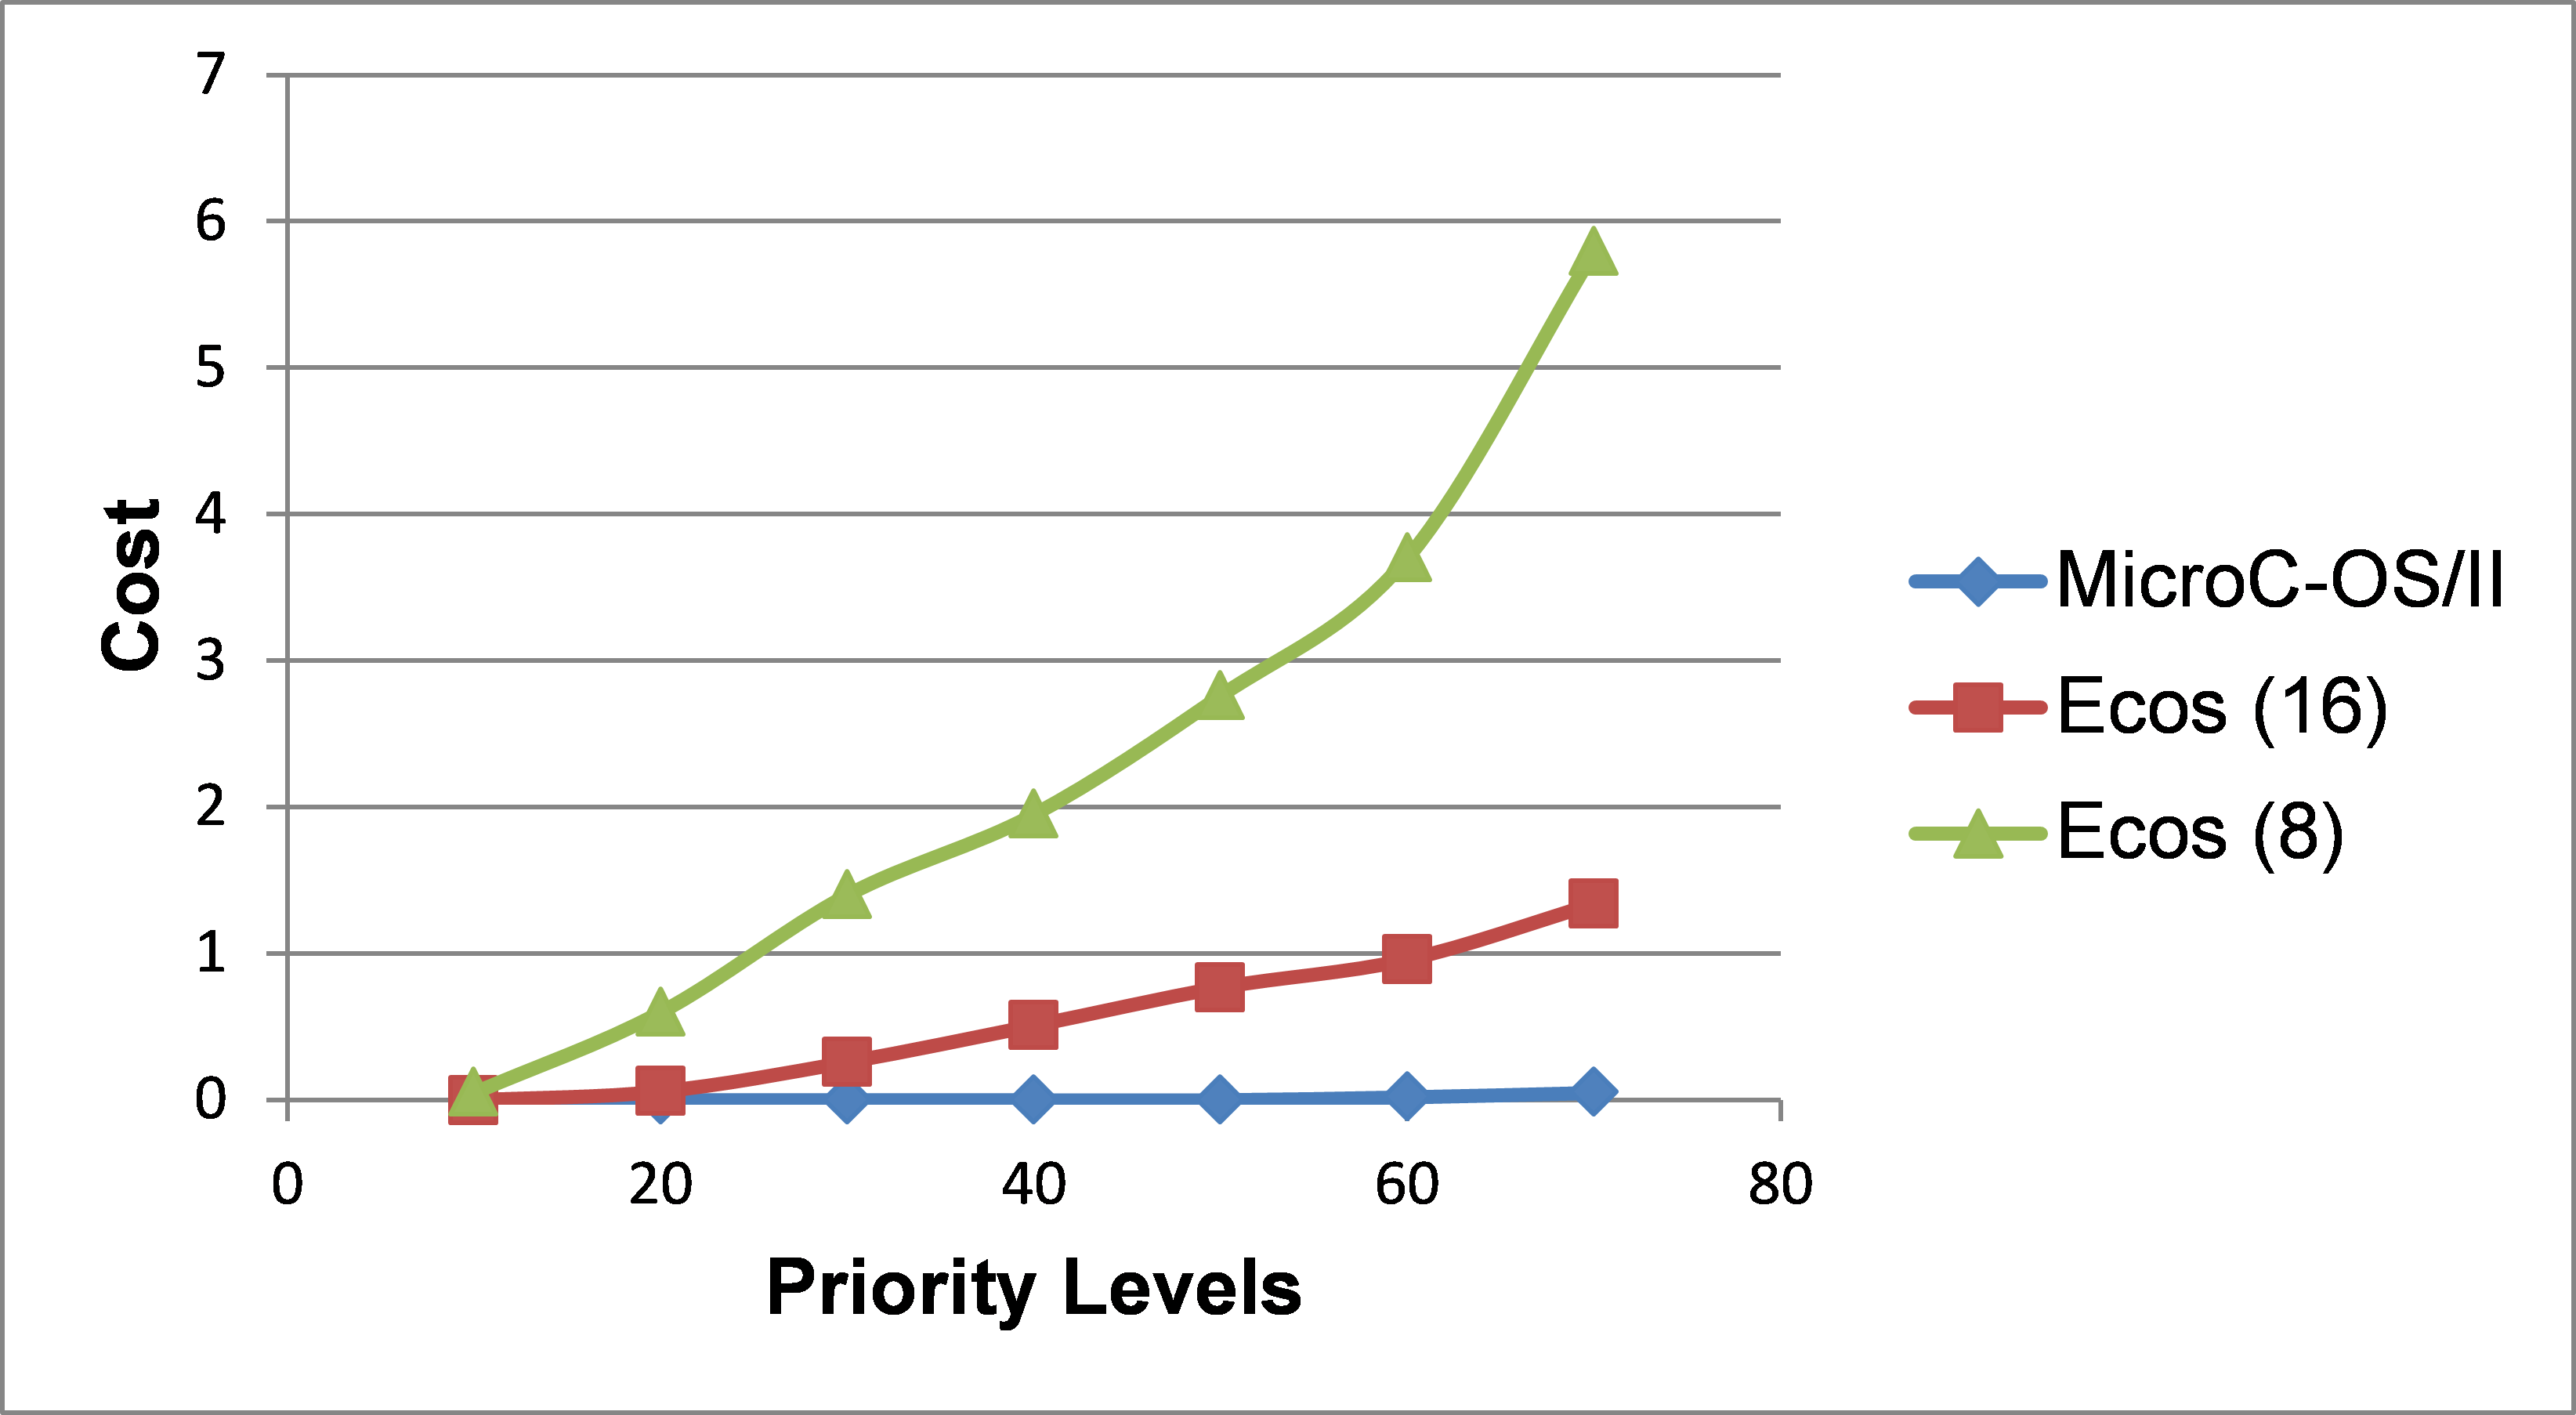
\includegraphics[width = 5cm]{Pic/largescale}
\label{Fig.cost}
}
\quad
\subfigure[Evaluation of the Resolution Time in Seconds]
{
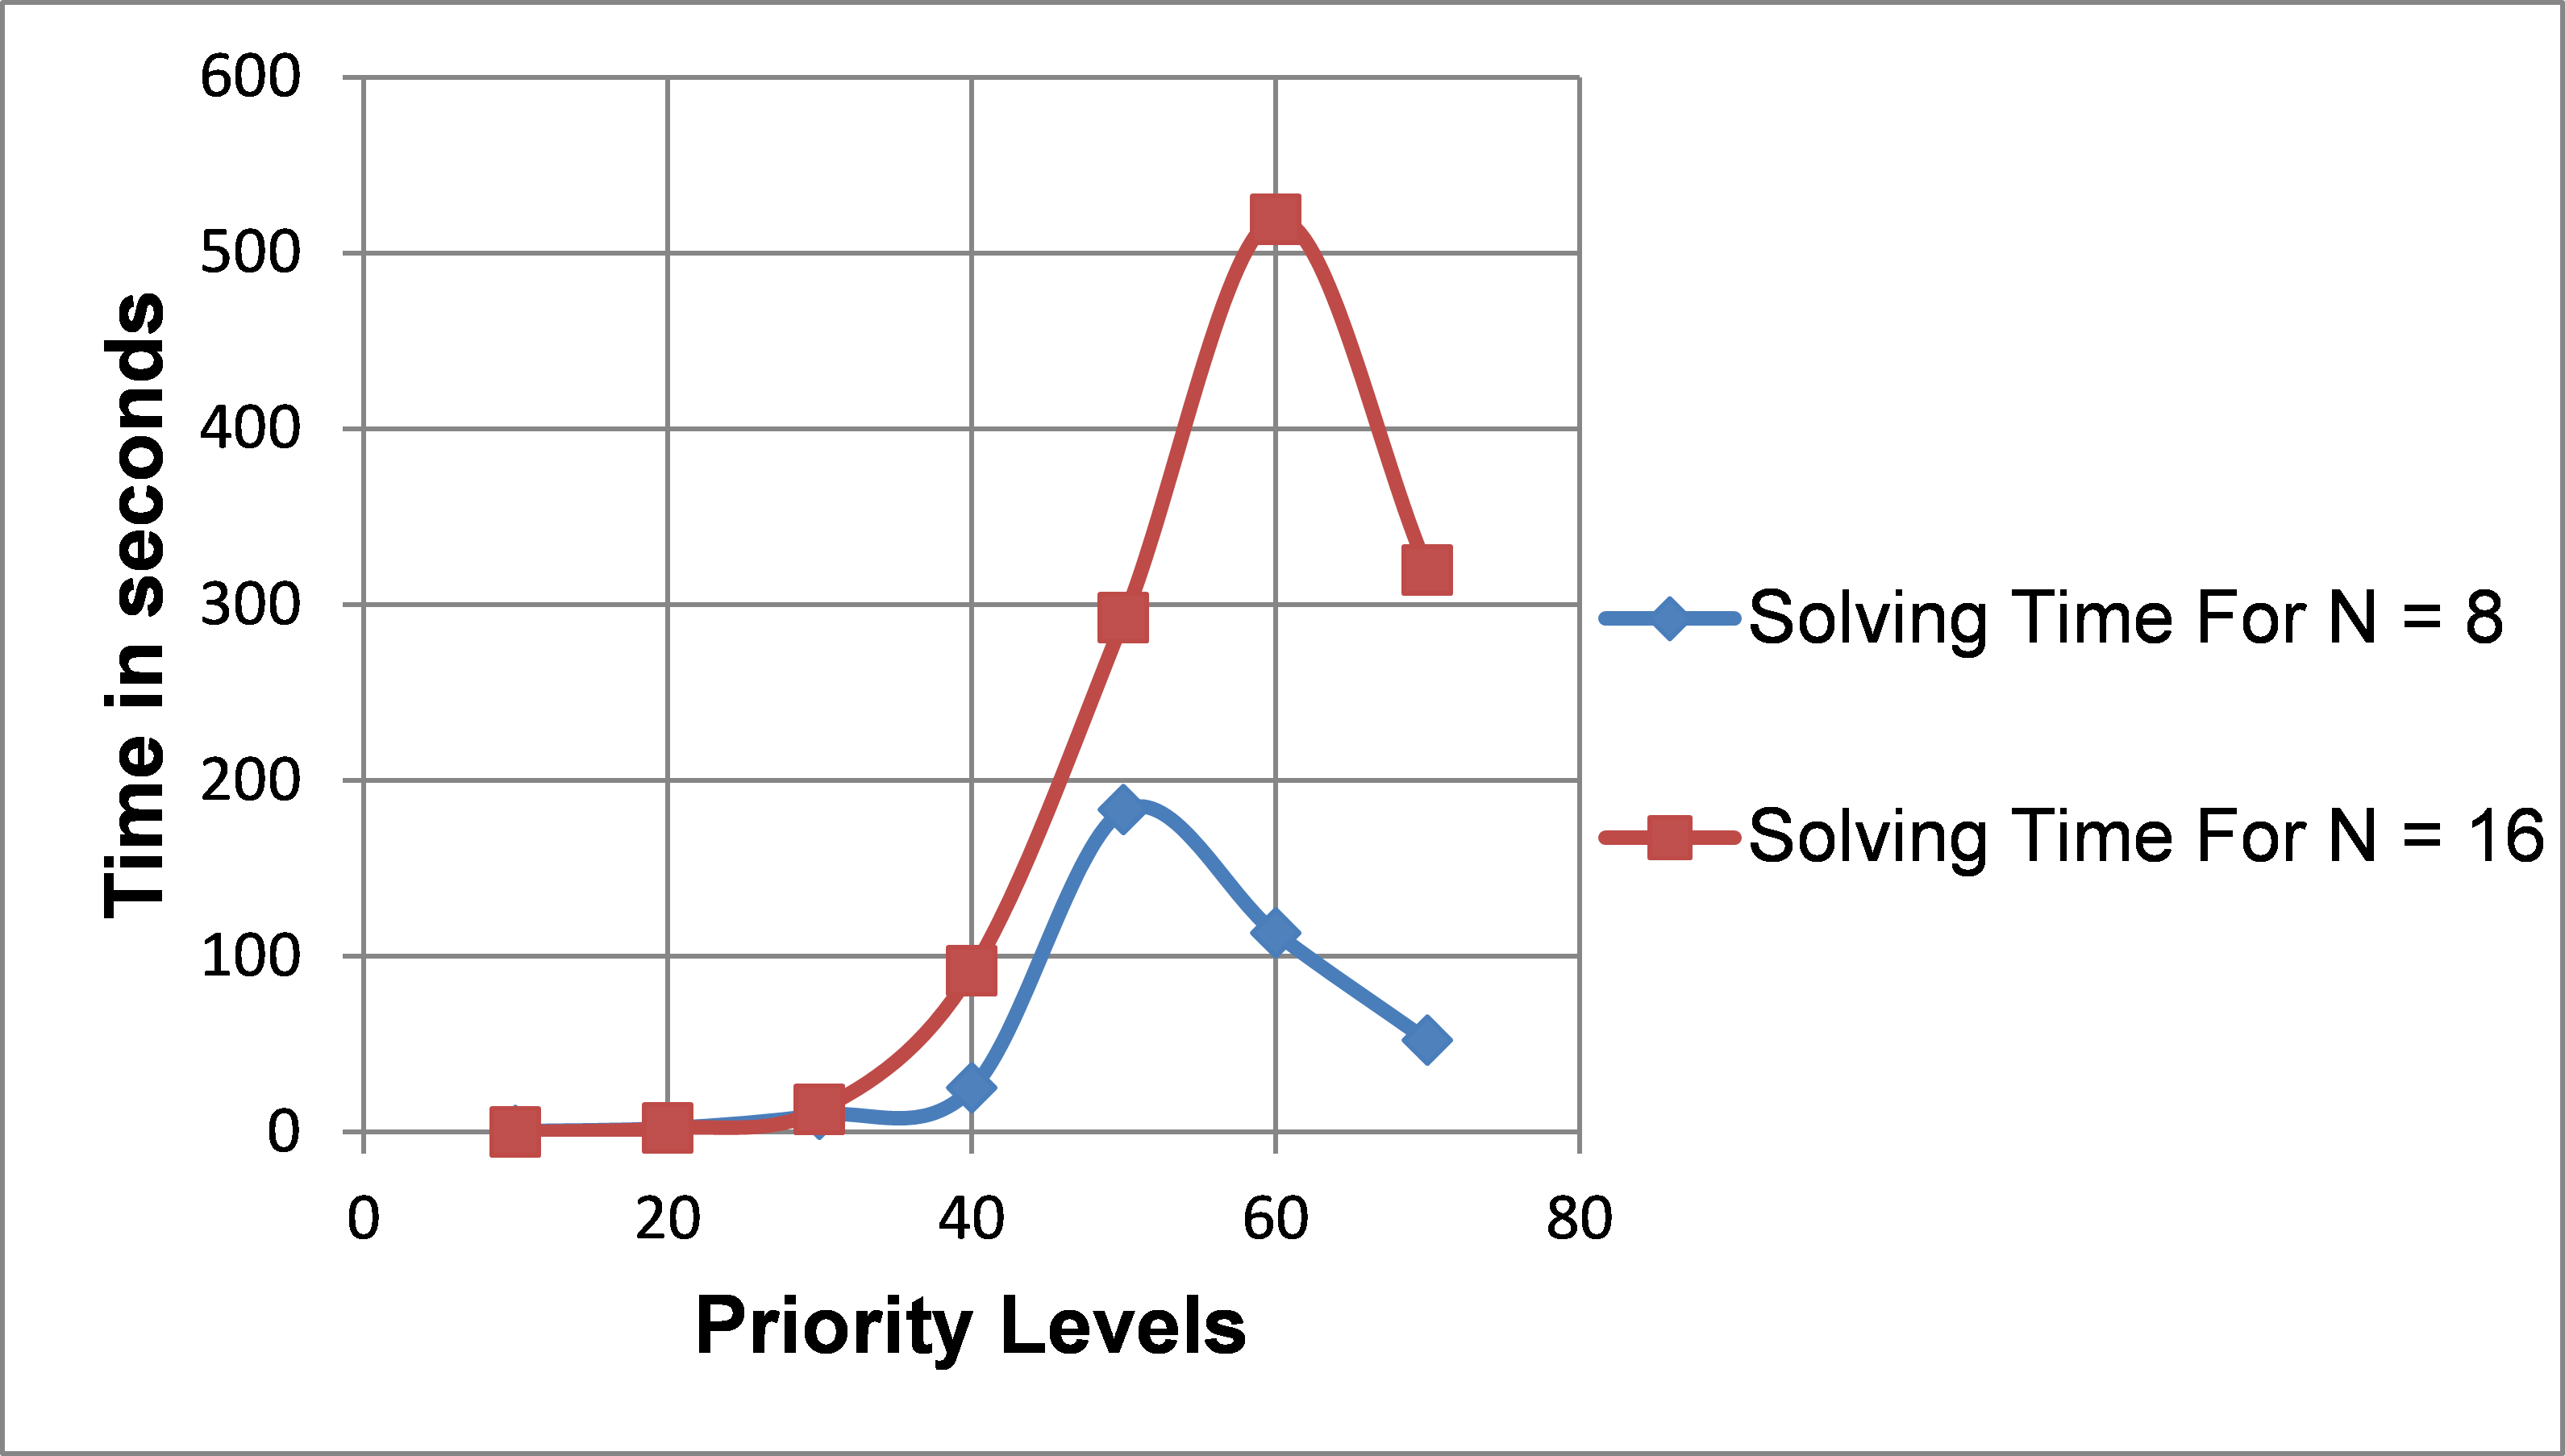
\includegraphics[width =5cm]{Pic/timeevaluation}
\label{Fig.time}
}
}
\caption{Evaluation of The Merge Pattern for Large Scale Applications}
\end{figure}
\\This evaluation shows that, in some cases, the deployment of a real time application requires some performance degradation, due the implementation constraints, to generate valid implementation models. This deployment cost is strongly influenced by the application and the target operating system. The merge pattern that we have proposed offers to the designer the possibility to estimate the performance loss for a particular application and a RTOS and thus provides a source of guidance for the selection of the appropriate operating system. 
\\Fig.4 (b) illustrates the variation of the resolution time in seconds. In fact, in this graph we evaluate the execution time of the linear program using CPLEX for different applications and for the Ecos Operating system configured respectively with 8 and 16 authorized applicative priority levels. From these graphics (Fig.4 (b)) we can conclude that the time required by the linear program to make decision is bounded even for large scale applications. The second conclusion is that this time depends strongly on the application and the target RTOS. In fact, it increases when the number of distinct priority levels in the architectural model increases and the number of priority levels authorized by the RTOS decreases. 
\section{Related Work}
Several approaches have been proposed to provide guidelines for the software development of RTES in a MDD context. In \cite{thomas}, the authors propose a generative process to transform an application deployed on one RTOS to another based on an explicit description of the involved RTOSs using SRM. This approach focuses especially on the portability requirement by proposing generic transformations enabling the deployment of the same application on several RTOSs. This work focuses on the structural aspect but makes the assumption that the deployment is always possible without any consideration of the potential difference between the semantics of RTOSs resources. The authors in \cite{wassim} extend the previous work by introducing behavioural information in platforms description. This approach focuses on the separation of concerns and portability while ensuring an automatic full code generation. To achieve that, the authors introduce behavioural patterns in platform models for a detailed description of the different services offered by the target platform. Indeed, these previously mentioned works do not consider real-time validation. 

In order to address real-time concerns, several works focus a specific standard and do not address the portability issue. In \cite{artisan}, the author extends the RT-UML profile to support the creation and validation of OSEK-compliant models. In \cite{icess05}, the authors use an OSEK-compliant abstract platform called SmartOSEK \cite{oseksmart} and define a set of transformation rules to create OSEK-compliant models from UML models. In addition, this approach enables the simulation of the resulting OSEK-compliant models and provides the designer with the results to optimize this model at design level. In \cite{isorc02}, the authors use RT-UML to annotate UML models describing real-time applications with timing properties. Then they identify the mapping rules between the resulting model and RT-Java as a target platform. The objective of this work is to properly propagate the real-time constraints into the RT-java specific model in order to validate them. From the other side, many existing works define MDD approaches to guide the design choices and generate architectural models satisfying timing properties. In \cite{marco} authors provides an approach to automatically generate the architectural model from the functional blocks. The focus of this work is to automate this generation and ensure optimized architectural models in terms of timing properties. In \cite{optimum} authors propose a MARTE-based methodology by introducing analysis from the functional level to guide the generation of a valid design model in terms of timing requirements. These works still keeping portability by ensuring platform-independent architectural models. However they in general end at the design level and do not focus on deployment issues. Hence, our approach aims at extending the latter methodology \cite{optimum} by focusing on the refinement toward implementation of the resulting design model. This work is a step toward providing portability and separation of concerns from one side and early verification of timing properties from the other side during the deployment process of a real-time application on a several RTOSs. 
%\section{Conclusion and Perspectives}
%In this paper we have proposed a model-driven approach to guide the transition from the design to the implementation model during the development of real-time applications. We have especially addressed the problem where the number of distinct priority levels used to validate the design model exceeds the number authorized by the RTOS. In that case, we have proposed a software pattern that we have called Distinct Priority Merge Pattern(DPMP) that automatically perform the re-factoring of the architectural model with the objective of solving the problem. The application of this pattern preserves the high level specification and the timing requirements while reducing the number of used distinct priority levels. Due to the complexity of this treatment, a MILP formulation of this pattern have been proposed. This formulation permits to confirm whether a solution exists for the problem and finds the better one in terms of processor utilization. 
%As perspective of this work, we aim at considering other problems such as timer granularity, equal priority levels, etc and proposing for each particular problem a software pattern to enrich our pattern base. In addition, we can extend this work by considering the behavioural aspect and thus other problems must be considered and consequently additional software pattern must be defined.
\section{Conclusion and Perspectives}
In this paper we have proposed a model-driven approach to guide the transition from the design to the implementation model during the development of real-time applications. We have especially addressed the problem where the number of distinct priority levels used to validate the design model exceeds the number authorized by the RTOS. In that case, we have proposed a software pattern that we have called Distinct Priority Merge Pattern(DPMP) that automatically perform the re-factoring of the architectural model with the objective of solving the problem. The application of this pattern preserves the high level specification and the timing requirements while reducing the number of used distinct priority levels. Due to the complexity of this treatment, a MILP formulation of this pattern have been proposed. This formulation permits to confirm whether a solution exists for the problem and finds the better one in terms of processor utilization. 

As perspective of this work, we aim at considering other problems such as timer granularity, equal priority levels, etc and proposing for each particular problem a software pattern to enrich our pattern base. In addition, we can extend this work by considering the behavioural aspect and thus other problems must be considered and consequently additional software pattern must be defined. 
\begin{thebibliography}{4}
%\bibitem{MDD} B. Schätz, A. Pretschner, F. Huber, J. Philipps. Model based  development of embedded systems, Lecture Notes in Computer Science,  vol 2426, 2002, Springer, 2002, pp.331-336.
\bibitem{optimum} C. Mraidha, S. Tucci-Piergiovanni, S. Gerard. Optimum: A MARTE-based methodology for Schedulability Analysis at Early Design Stages. In proceeding of the Third IEEE international workshop UML and Formal Methods (UML\&FM 2010). Shanghai, China
\bibitem{cheddar}F. Singhoff, J. Legrand, L. Nana, and L. Marcé. Cheddar: a Flexible Real Time Scheduling Framework. International ACM SIGADA Conference, Atlanta, November 2004. 
\bibitem{SEAA}R. Mzid, Ch. Mraidha, J-P. Babau, M. Abid. A MDD Approach for RTOS Integration on Valid Real-Time Design Model. The 38th Euromicro Conference On software Engineering and Advanced Applications (SEAA’12), Cesme, Izmir, Turkey, September 2012. 
\bibitem{models}R. Mzid, Ch. Mraidha, J-P. Babau, M. Abid. Real-Time Design Models to RTOS-Specific Models Refinement Verification.  The 5th International Workshop on Model Based Architecting and construction of Embedded Systems ACES-MB 2012 in Conjunction with the 15th International Conference  on Model Driven Engineering Languages \& Systems MODELS 2012, Innsbruck, Austria, September 2012. 
\bibitem{SRM}Object Management Group, UML Profile for MARTE: Modeling and Analysis of Real-Time Embedded Systems, Object Management Group, Inc., September 2010, OMG document number: ptc/2010-08-32
\bibitem{PCP} J. B. Goodenough and L. Sha. The priority ceiling protocol: A method for minimizing the blocking of high priority Ada tasks, volume 8.ACM, 1988
\bibitem{RMA} M. H. Klein, T. Ralya, B. Pollak, R. Obenza, and M. G. Harbour.A practitioner’s handbook for real-time analysis. Kluwer Academic Publishers, 1993.
\bibitem{microc} Jean J. Labrosse. MicroC/OS-II The Real-Time Kernel 
\bibitem{ecos} Anthony. J. MASSA Embedded Software Development with Ecos
\bibitem{thomas} F. Thomas, J. Delatour, F. Terrier, and S. Gerad. Toward a framework for explicit platform-based transformations. In Proceeding of the 11th IEEE Symposium on Object Oriented Real-Time Distributed Computing (ISORC). Orlondo, Florida, USA, May 2008.
\bibitem{wassim} W. E. H. Chehade, A. Radermacher, F. Terrier, B. Selic, and S. Gerard, “A model-driven framework for the development of portable real-time embedded systems,” in Proceedings of the 16th IEEE International Conference on Engineering of Complex Computer Systems. Las Vegas, Nevada, USA: IEEE Computer Society, 2011, pp. 45–54.
\bibitem{marco} C. Bartolini, G. Lipari, and M. D. Natale, “From functional blocks to the synthesis of the architectural model
in embedded real-time applications,” in Proc. IEEE Real Time and Embedded Technology and Applications Symposium (RTAS), 2005, pp. 458–467.
\bibitem{artisan} A. Moore. Extending the RT-profile le to support the OSEK
infrastructure. In Proceedings of the 5th IEEE International Symposium on Object-Oriented Real-Time Distributed Computing, pages 341–347, Washington, DC, Apr. 2002.
\bibitem{icess05}G. Yang, M. Zhao, L. Wang, and Z. Wu, "Model-based Design and Verification of Automotive Electronics Compliant with OSEK/VDX," presented at The Secend International Conference on Embedded Software and System (ICESS), Xi'an, 2005.
\bibitem{oseksmart} M. Zhao, Z. Wu, G. Yang, L. Wang, and W. Chen,"SmartOSEK: A Dependable Platform for Automobile Electronics," The First International Conference on Embedded Software and System, vol. Springer-Verlag GmbH ISSN: 0302-9743, pp. 437, 2004.
\bibitem{isorc02} Becker, L.B.; Holtz, R.; Pereira, C.E. On Mapping RTUML Specifications to RT-Java API: Bridging the Gap. In: 5th IEEE International Symposium on Object-Oriented Real-Time Distributed Computing, Washington, USA, 2002. p. 348-355

%\bibitem{osek}OSEK/VDX, "OSEK/VDX Operating System Specification Version 2.2.2," 2004.

%\bibitem{jour} Smith, T.F., Waterman, M.S.: Identification of Common Molecular
%Subsequences. J. Mol. Biol. 147, 195--197 (1981)

%\bibitem{lncschap} May, P., Ehrlich, H.C., Steinke, T.: ZIB Structure Prediction Pipeline:
%Composing a Complex Biological Workflow through Web Services. In: Nagel,
%W.E., Walter, W.V., Lehner, W. (eds.) Euro-Par 2006. LNCS, vol. 4128,
%pp. 1148--1158. Springer, Heidelberg (2006)

%\bibitem{book} Foster, I., Kesselman, C.: The Grid: Blueprint for a New Computing
%Infrastructure. Morgan Kaufmann, San Francisco (1999)

%\bibitem{proceeding1} Czajkowski, K., Fitzgerald, S., Foster, I., Kesselman, C.: Grid
%Information Services for Distributed Resource Sharing. In: 10th IEEE
%International Symposium on High Performance Distributed Computing, pp.
%181--184. IEEE Press, New York (2001)

%\bibitem{proceeding2} Foster, I., Kesselman, C., Nick, J., Tuecke, S.: The Physiology of the
%Grid: an Open Grid Services Architecture for Distributed Systems
%Integration. Technical report, Global Grid Forum (2002)

%\bibitem{url} National Center for Biotechnology Information, %\url{http://www.ncbi.nlm.nih.gov}

\end{thebibliography}

\end{document}

%\\We consider now a second example by modifying just the execution time of the tasks $T_1$ and $T_2$. The resulting model is $M =\{T_1,T_2,T_3,T_4\}$ with  $T_1=(1,2,10,10,0,f_1)$, $T_2=(2,3,20,20,0,f_2)$, $T_3=(3,2,30,30,0,f_3)$ and $T_4=(4,1,60,60,0,f_4)$. The initial processor utilization for this model is 43,33\%. For this example also 5 solutions are possible and they are presented in Table 2. 
%\begin{table}
%\caption{Example 2: Possible Solutions and Utilization estimation}
%\label{table1}
%\centering
 %  \begin{tabular}{ | l || c |}
  %   \hline
   %  Possible Solutions & Utilization \\
    % \hline
    % $M_1 =(\{T_1,T_2\},\{T_3,T_4\}$) &  60\% \\
     %\hline
     %$M_2 =(\{T_1,T_3\},\{T_2,T_4\}$)& 60\% \\
     %\hline
     %$M_3 = (\{T_1,T_2,T_3\},T_4$) & 71,67\%\\
     %\hline
     %$M_4=(T_2,\{T_1,T_3,T_4\})$ & 65\% \\
     %\hline
     %$M_5= (T_3,\{T_1,T_2,T_4\})$ & 66,67\% \\
     %\hline
   %\end{tabular}
%\end{table}  
%\\Similarly the solution found for this example with the heuristic method is $M_3$ and we can easily conclude that for this particular example this solution is the worst in terms of processor utilization. From these considerations, an appropriate method must be considered to solve this problem. This method must be able to confirm whether solution for each particular problem (application and RTOS) exists. In addition, when many solutions are available, this method should find one which costs less performance degradation. In next section, we propose a MILP formulation of this problem.  

%Any of these approaches treats portability and real-time validation at the same time during the deployment phase. Therefore, our approach aims at extending the work in \cite{optimum} by adding 
%is a step toward providing portability and separation of concerns from one side and early verification of timing properties from the other side during the deployment process.  
%To achieve that, they make assumptions about the underlying RTOS to generate models and verify the timing properties. For instance, the authors in \cite{optimum} suppose that the RTOS provides a fixed priority scheduling policy whereas in \cite {marco} the authors consider an EDF one.

%Similarly to our approach, the authors in \cite{iceccs12} focus on portability and real-time aspect. To this end, they define a set of refinement rules using design patterns to create intermediate models between the design and the implementation level and enable validation at each model to get accurate analysis results. Unlike our approach, this work focus especially on behaviour refinement based on an abstract execution platform. 
